\documentclass[9pt, aspectratio=169]{beamer}

\usetheme{ugoe}
\usepackage{setspace}  %% Zur Setzung des Zeilenabstandes
\usepackage{blindtext}
\usepackage{float}
\usepackage{svg}
\usepackage{babel}     %% Sprachen-Unterstuetzung
\usepackage{calc}      %% ermoeglicht Rechnen mit Laengen und Zaehlern
\usepackage[T1]{fontenc}       %% Unterstutzung von Umlauten etc.
\usepackage[utf8]{inputenc}  %% 
%% in aktuellem Linux & MacOS X wird standardmaessig UTF8 kodiert!
%\usepackage[utf8]{inputenc}    %% Wenn latin1 nicht geht ...
\usepackage{amsmath,amssymb} %% zusaetzliche Mathe-Symbole
\usepackage{lmodern} %% type1-taugliche CM-Schrift als Variante zur
                     %% "normalen" EC-Schrift
%% Paket fuer bibtex-Datenbanken
\usepackage[comma,numbers,sort&compress]{natbib}
\bibliographystyle{datenbank}
% \bibliographystyle{plainnat}

\newcommand{\tabheadfont}[1]{\textbf{#1}} %% Tabellenkopf in Fett
\usepackage{booktabs}                      %% Befehle fuer besseres Tabellenlayout
\usepackage{longtable}                     %% umbrechbare Tabellen
\usepackage{array}                         %% zusaetzliche Spaltenoptionen

%% umfangreiche Pakete fuer Symbole wie \micro, \ohm, \degree, \celsius etc.
\usepackage{textcomp,gensymb}
%\usepackage{SIunits} %% Korrektes Setzen von Einheiten
\usepackage{units}   %% Variante fuer Einheiten
\usepackage[pdfstartview=FitH,      % Oeffnen mit fit width
            breaklinks=true,        % Umbrueche in Links, nur bei pdflatex default
            bookmarksopen=true,     % aufgeklappte Bookmarks
            bookmarksnumbered=true  % Kapitelnummerierung in bookmarks
            ]{hyperref}

\usepackage{amsmath}
\usepackage{scrhack}
\usepackage[table]{xcolor}

\newcolumntype{L}[1]{>{\raggedright\arraybackslash}p{#1}}
\newcolumntype{C}[1]{>{\centering\arraybackslash}p{#1}}
\newcolumntype{R}[1]{>{\raggedleft\arraybackslash}p{#1}}
\newcolumntype{?}{!{\vrule width .1mm}}
\newcolumntype{V}{!{\vrule width .3mm}}
% ==================================================
% ==========  FORMATING   ==========================
% ==================================================
\newcommand*{\highl}[1]{\textbf{\color{ugoelogodark}#1}}


% ==================================================
% ==========  ALIASES  =============================
% ==================================================
\newcommand{\HWW}       {\mbox{$H\rightarrow WW^*$}\xspace}
\newcommand{\ttHWW}     {\mbox{$t\bar{t}(H\rightarrow WW^*)$}\xspace}
\newcommand{\spanet}	{\texttt{SPA-Net}\xspace}
\newcommand{\spanets}	{\texttt{SPA-Net}'s\xspace}

\newcommand{\ttbar}      {\mbox{$t\bar{t}$}\xspace}
\newcommand{\ttbarW}     {\mbox{$t\bar{t}W$}\xspace}
\newcommand{\ttbarZ}     {\mbox{$t\bar{t}Z$}\xspace}
\newcommand{\ttbarH}     {\mbox{$t\bar{t}H$}\xspace}

\newcommand{\tquark}   	{top quark\xspace}
\newcommand{\tquarks}   {top quarks\xspace}
\newcommand{\bquark}   	{bottom quark\xspace}
\newcommand{\bquarks}   {bottom quarks\xspace}
\newcommand{\zboson}   	{$Z$-boson\xspace}
\newcommand{\zbosons}  	{$Z$-bosons\xspace}
\newcommand{\wboson}   	{$W$-boson\xspace}
\newcommand{\wbosons}  	{$W$-bosons\xspace}
\newcommand{\zwboson}   {$Z$/$W$-boson\xspace}
\newcommand{\zwbosons}  {$Z$/$W$-bosons\xspace}

\newcommand{\cern}      {{C{\textsc{ern}}}\xspace}
\newcommand{\atlas}     {{A{\textsc{tlas}}}\xspace}
\newcommand{\desy}     {{D{\textsc{esy}}}\xspace}
\newcommand{\lhc}       {{L{\textsc{hc}}}\xspace}
\newcommand{\lhcb}      {{L{\textsc{hc}}}{\scriptsize{b}}\xspace}
\newcommand{\runi}      {Run~I\xspace}
\newcommand{\runii}     {Run~II\xspace}

\newcommand{\dzero}      {D\O\xspace}
\newcommand{\cdf}        {CDF\xspace}
\newcommand{\uubar}      {\mbox{u\textoverline{u}}\xspace}
\newcommand{\ddbar}      {\mbox{d\textoverline{d\kern0.05em}\kern-0.05em}\xspace}
\newcommand{\ccbar}      {\mbox{c\kern-0.02em\textoverline{\kern0.02em{}c\kern0.02em}\kern-0.02em}\xspace}
\newcommand{\ssbar}      {\mbox{s\kern-0.02em\textoverline{\kern0.02em{}s\kern0.02em}\kern-0.02em}\xspace}
\newcommand{\bbbar}      {\mbox{b\kern-0.05em\textoverline{\kern0.05em{}b}}\xspace}
\newcommand{\ccbarbold}  {\mbox{\textbf{c\kern-0.02em\textboldoverline{\kern0.02em{}c\kern0.02em}\kern-0.02em}}\xspace}
\newcommand{\ttbarbold}  {\mbox{\textbf{t\kern-0.05em\textboldoverline{\kern0.05em{}t}}}\xspace}
\newcommand{\bbbarbold}  {\mbox{\textbf{b\kern-0.05em\textboldoverline{\kern0.05em{}b}}}\xspace}

\newcommand{\wjets}      {\mbox{W\,+\,4\;jets}\xspace}
\newcommand{\pttbar}     {\mbox{p\textsubscript{\ttbar}}\xspace}
\newcommand{\pwjets}     {\mbox{p\textsubscript{W\,+\,4\;jets}}\xspace}
\newcommand{\ljets}      {\mbox{$\ell$\,+\,jets}\xspace}
\newcommand{\ejets}      {\mbox{e\,+\,jets}\xspace}
\newcommand{\mujets}     {\mbox{$\mu$\,+\,jets}\xspace}
\newcommand{\ttjets}     {\mbox{\ttbar{}\,+\,jets}\xspace}
\newcommand{\ttljets}    {\mbox{\ttbar{}\,+\,light jets}\xspace}
\newcommand{\ttlight}    {\mbox{\ttbar{}\,+\,light}\xspace}
\newcommand{\ttc}        {\mbox{\ttbar{}\,+\,c}\xspace}
\newcommand{\ttb}        {\mbox{\ttbar{}\,+\,b}\xspace}
\newcommand{\wt}         {\mbox{Wt}\xspace}

\newcommand{\ttx}        {\mbox{\ttbar{}X}\xspace}
\newcommand{\ttv}        {\mbox{\ttbar{}V}\xspace}
\newcommand{\thiggs}     {\mbox{tH}\xspace}
\newcommand{\tth}        {\mbox{\ttbar{}H}\xspace}
\newcommand{\hbb}        {\mbox{H\,$\rightarrow$\,\bbbar}\xspace}
\newcommand{\thbb}       {\mbox{\thiggs{}(\hbb)}\xspace}
\newcommand{\tthbb}      {\mbox{\tth{}(\hbb)}\xspace}
\newcommand{\tthgam}     {\mbox{\tth{}(H\,$\rightarrow$\,$\gamma\gamma$)}\xspace}
\newcommand{\ttbb}       {\mbox{\ttbar{}\,+\,\bbbar}\xspace}

\newcommand{\thiggsbold} {\mbox{\textbf{tH}}\xspace}
\newcommand{\tthbold}    {\mbox{\ttbarbold{}\textbf{H}}\xspace}
\newcommand{\hbbbold}    {\mbox{\textbf{H}\,$\boldsymbol{\rightarrow}$\,\bbbarbold}\xspace}
\newcommand{\thbbbold}   {\mbox{\thiggsbold{}\textbf{(}\hbbbold{}\textbf{)}}\xspace}
\newcommand{\tthbbbold}  {\mbox{\tthbold{}\textbf{(}\hbbbold{}\textbf{)}}\xspace}

\newcommand{\thiggstitle}{\mbox{tH}\xspace}
\newcommand{\tthtitle}   {\mbox{t\kern-0.02em$\overline{\kern0.05em{}\mathrm{t}}$H}\xspace}
\newcommand{\hbbtitle}   {\mbox{H\,$\rightarrow$\,b\kern-0.05em$\overline{\kern0.05em{}\mathrm{b}}$}\xspace}
\newcommand{\tthbbtitle} {\mbox{\tthtitle{}(\hbbtitle)}\xspace}

\newcommand{\pt}         {\mbox{$p_{\kern0.1em\mathrm{T}}$}\xspace}
\newcommand{\mathpt}     {p_{\kern0.1em\mathrm{T}}}

\usepackage{bbding}
\usepackage{pifont}

\definecolor{highlighter}{RGB}{0,95,155}

\title{Studies of \ttHWW with SPA-Net \& Neutrino Weighting}
\date{08.04.2024}
\author{Ireas Tom Raschke}
\institute{II.\ Physikalisches Institut, Univ.\ of Göttingen}
\supervisor{Prof. Arnulf Quadt} %Dr. Baptiste Ravina, Steffen Korn, Chris Scheulen
%\conference{}

% \addtocounter{framenumber}{-1} 

% =======================================================
% =======  START  =======================================
% =======================================================
\begin{document}
\begin{frame}
	\fontsize{11pt}{14pt}\selectfont
	\titlepage
\end{frame}

\begin{frame}{Project}{Overview}
	\begin{minipage}{.58\textwidth}
		\begin{itemize}
			\item full event reconstruction of \ttHWW
			\begin{itemize}
				\item unanalysed channel
				\begin{itemize}
					\item only leptonic channel previously done
				\end{itemize}  
				\item challenging topology $\Rightarrow$ modern techniques
				\begin{itemize}
					\item \spanet (machine learning)
					\item neutrino weighting
				\end{itemize}  
			\end{itemize}
			\item main measurement
			\begin{itemize}
				\item inclusive cross-section / differential STXS
				\item performance of new techniques
				\item $tH$ coupling, \HWW spin correlation, ... (difficult)
			\end{itemize}
		\end{itemize}
	\end{minipage}
	\begin{minipage}{.4\textwidth}
		\begin{figure}
			\centering
			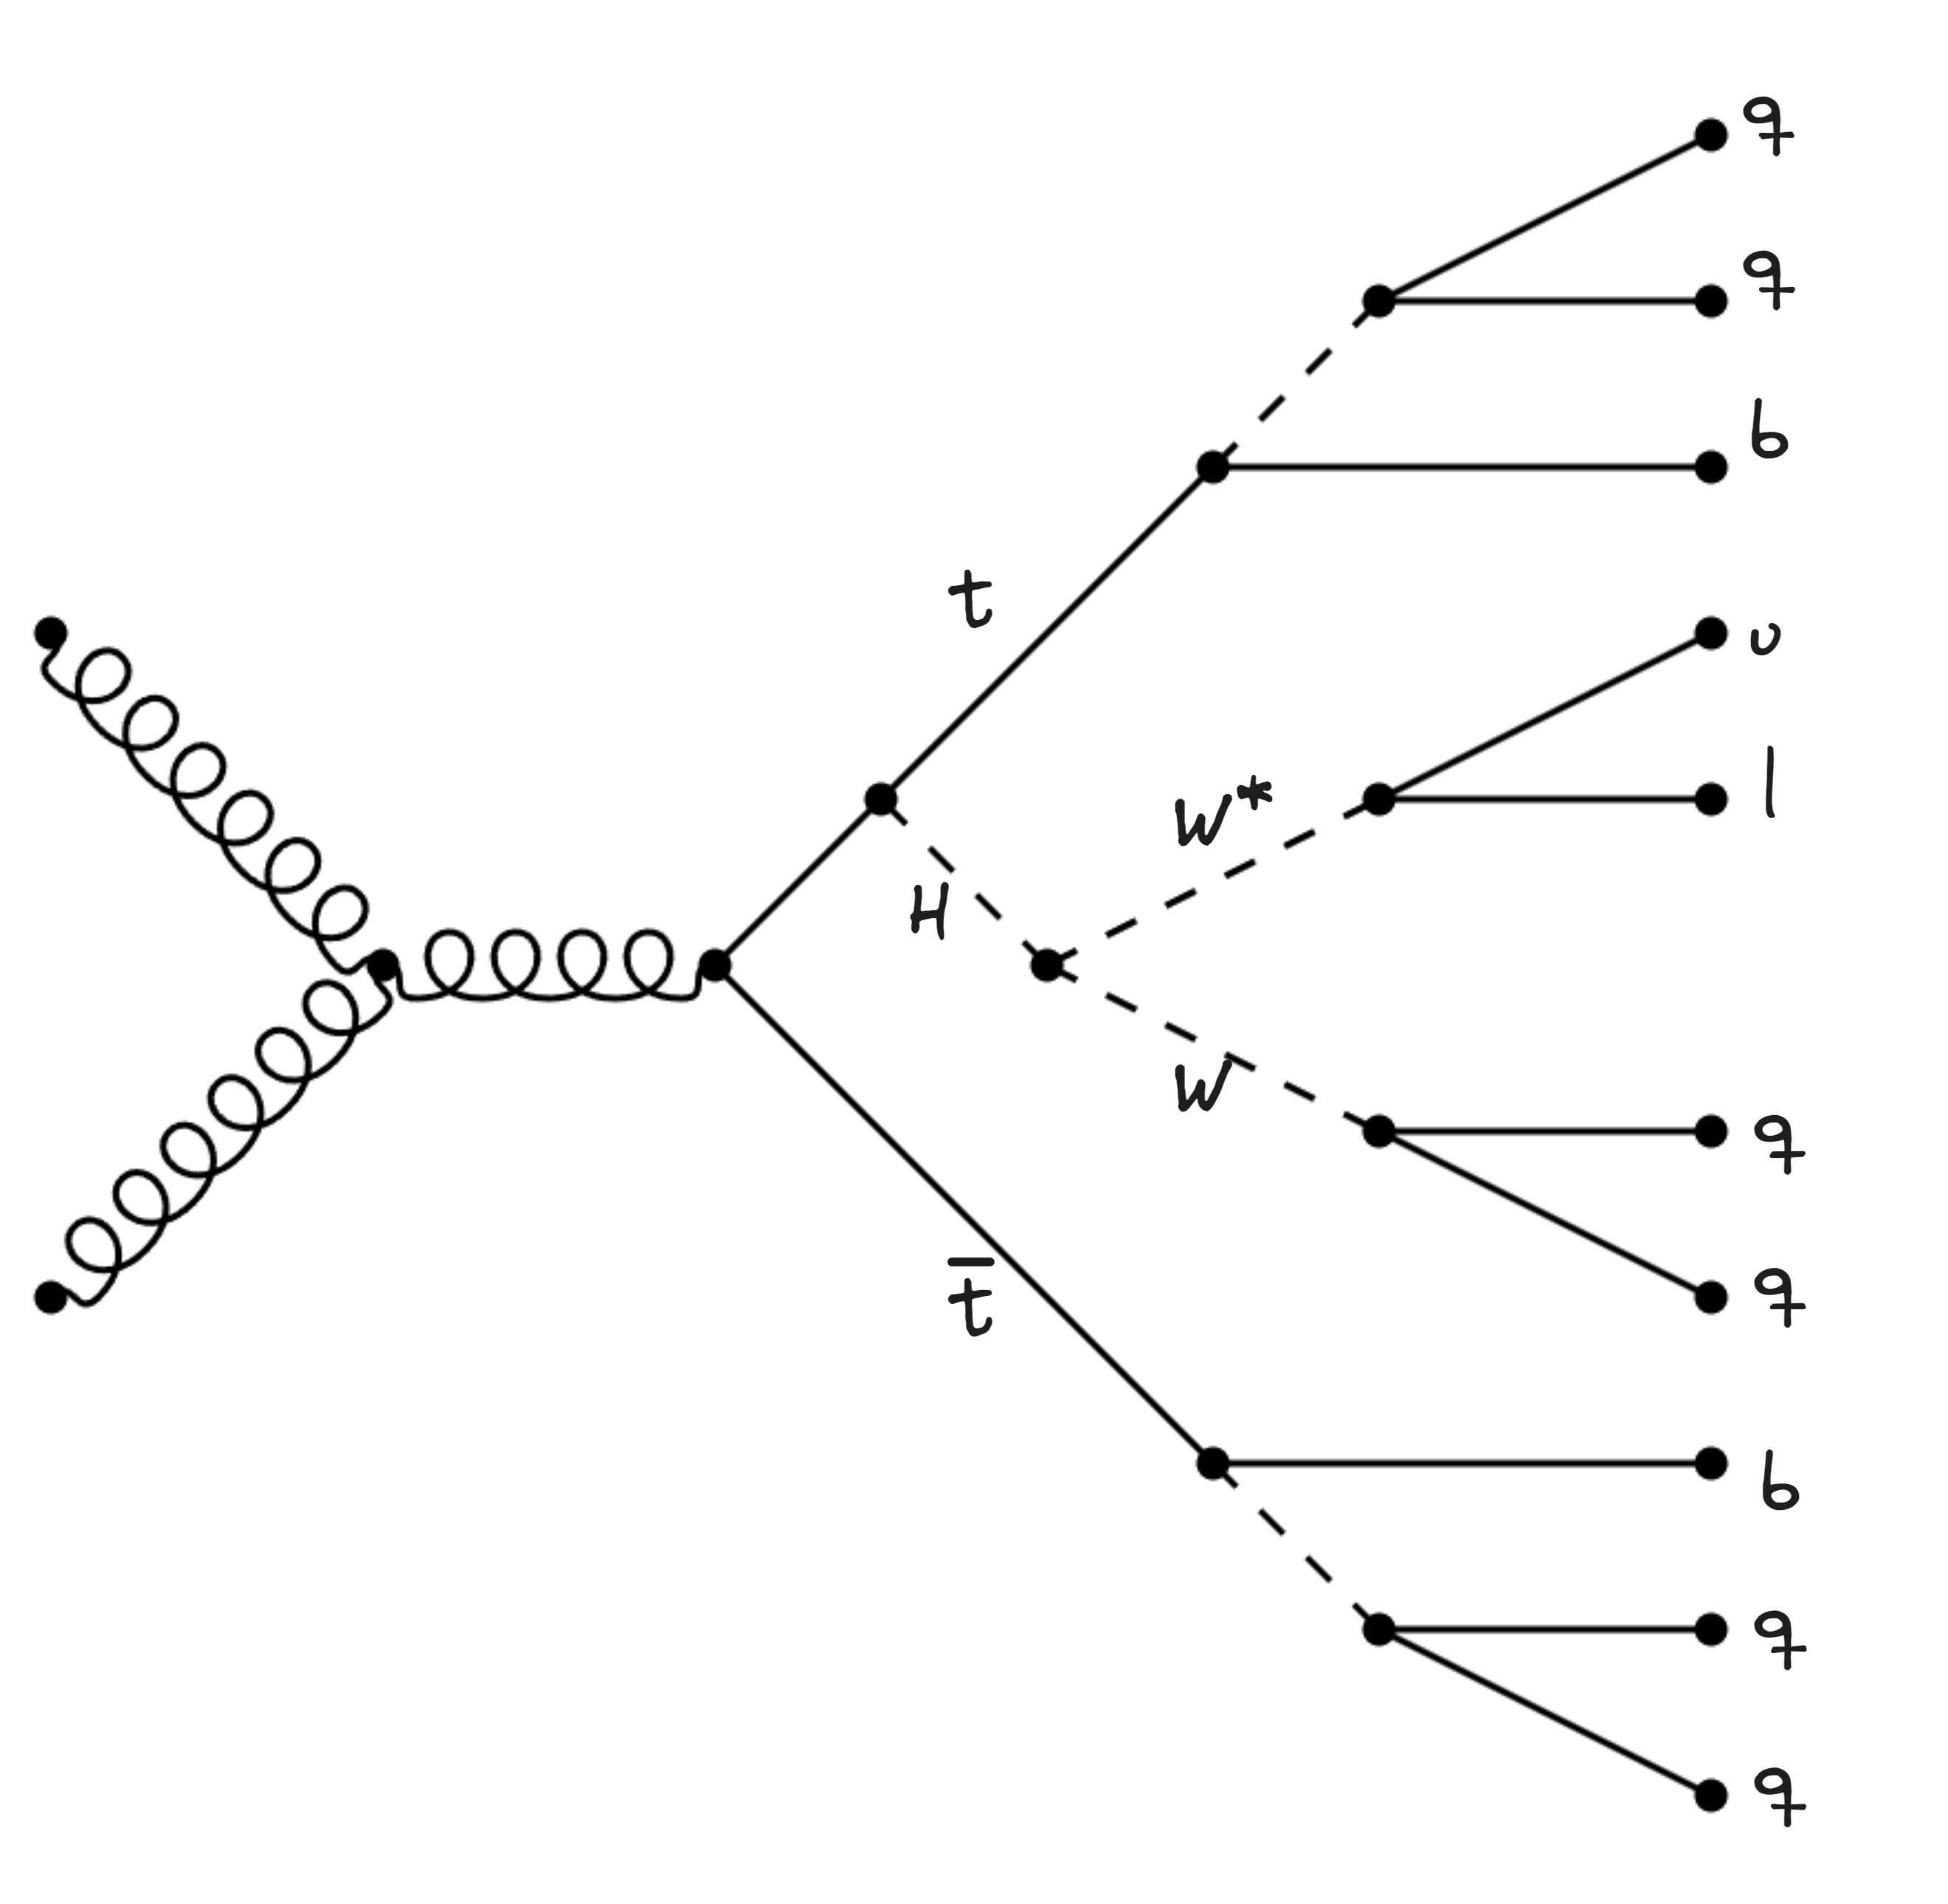
\includegraphics[width=\textwidth]{feynman_diagrams/tthww_undivided.excalidraw.png}
		\end{figure}
	\end{minipage}       	
\end{frame}

\begin{frame}{Event Topology}{Into the Unknown}
	\begin{minipage}{.58\textwidth}
		\begin{itemize}
			\item target \ttHWW events
			\begin{itemize}
				\item fully hadronic \ttbar
				\item $H$ radiated from \ttbar
				\item semi-leptonic \HWW$\rightarrow (l\nu)(qq)$
        	\end{itemize}
			\item resonance particles ($W$,$H$,$t$)
			\begin{itemize}
				\item decay before detection
				\item reconstruct from final state
			\end{itemize} 
			\item final state
			\begin{itemize}
				\item 6(2$b$) quarks from \ttbar
				\item 2 quarks from \HWW
				\item 1 lepton-neutrino pair from \HWW 
			\end{itemize}
		\end{itemize}
	\end{minipage}
	\begin{minipage}{.4\textwidth}
		\begin{figure}
			\centering
			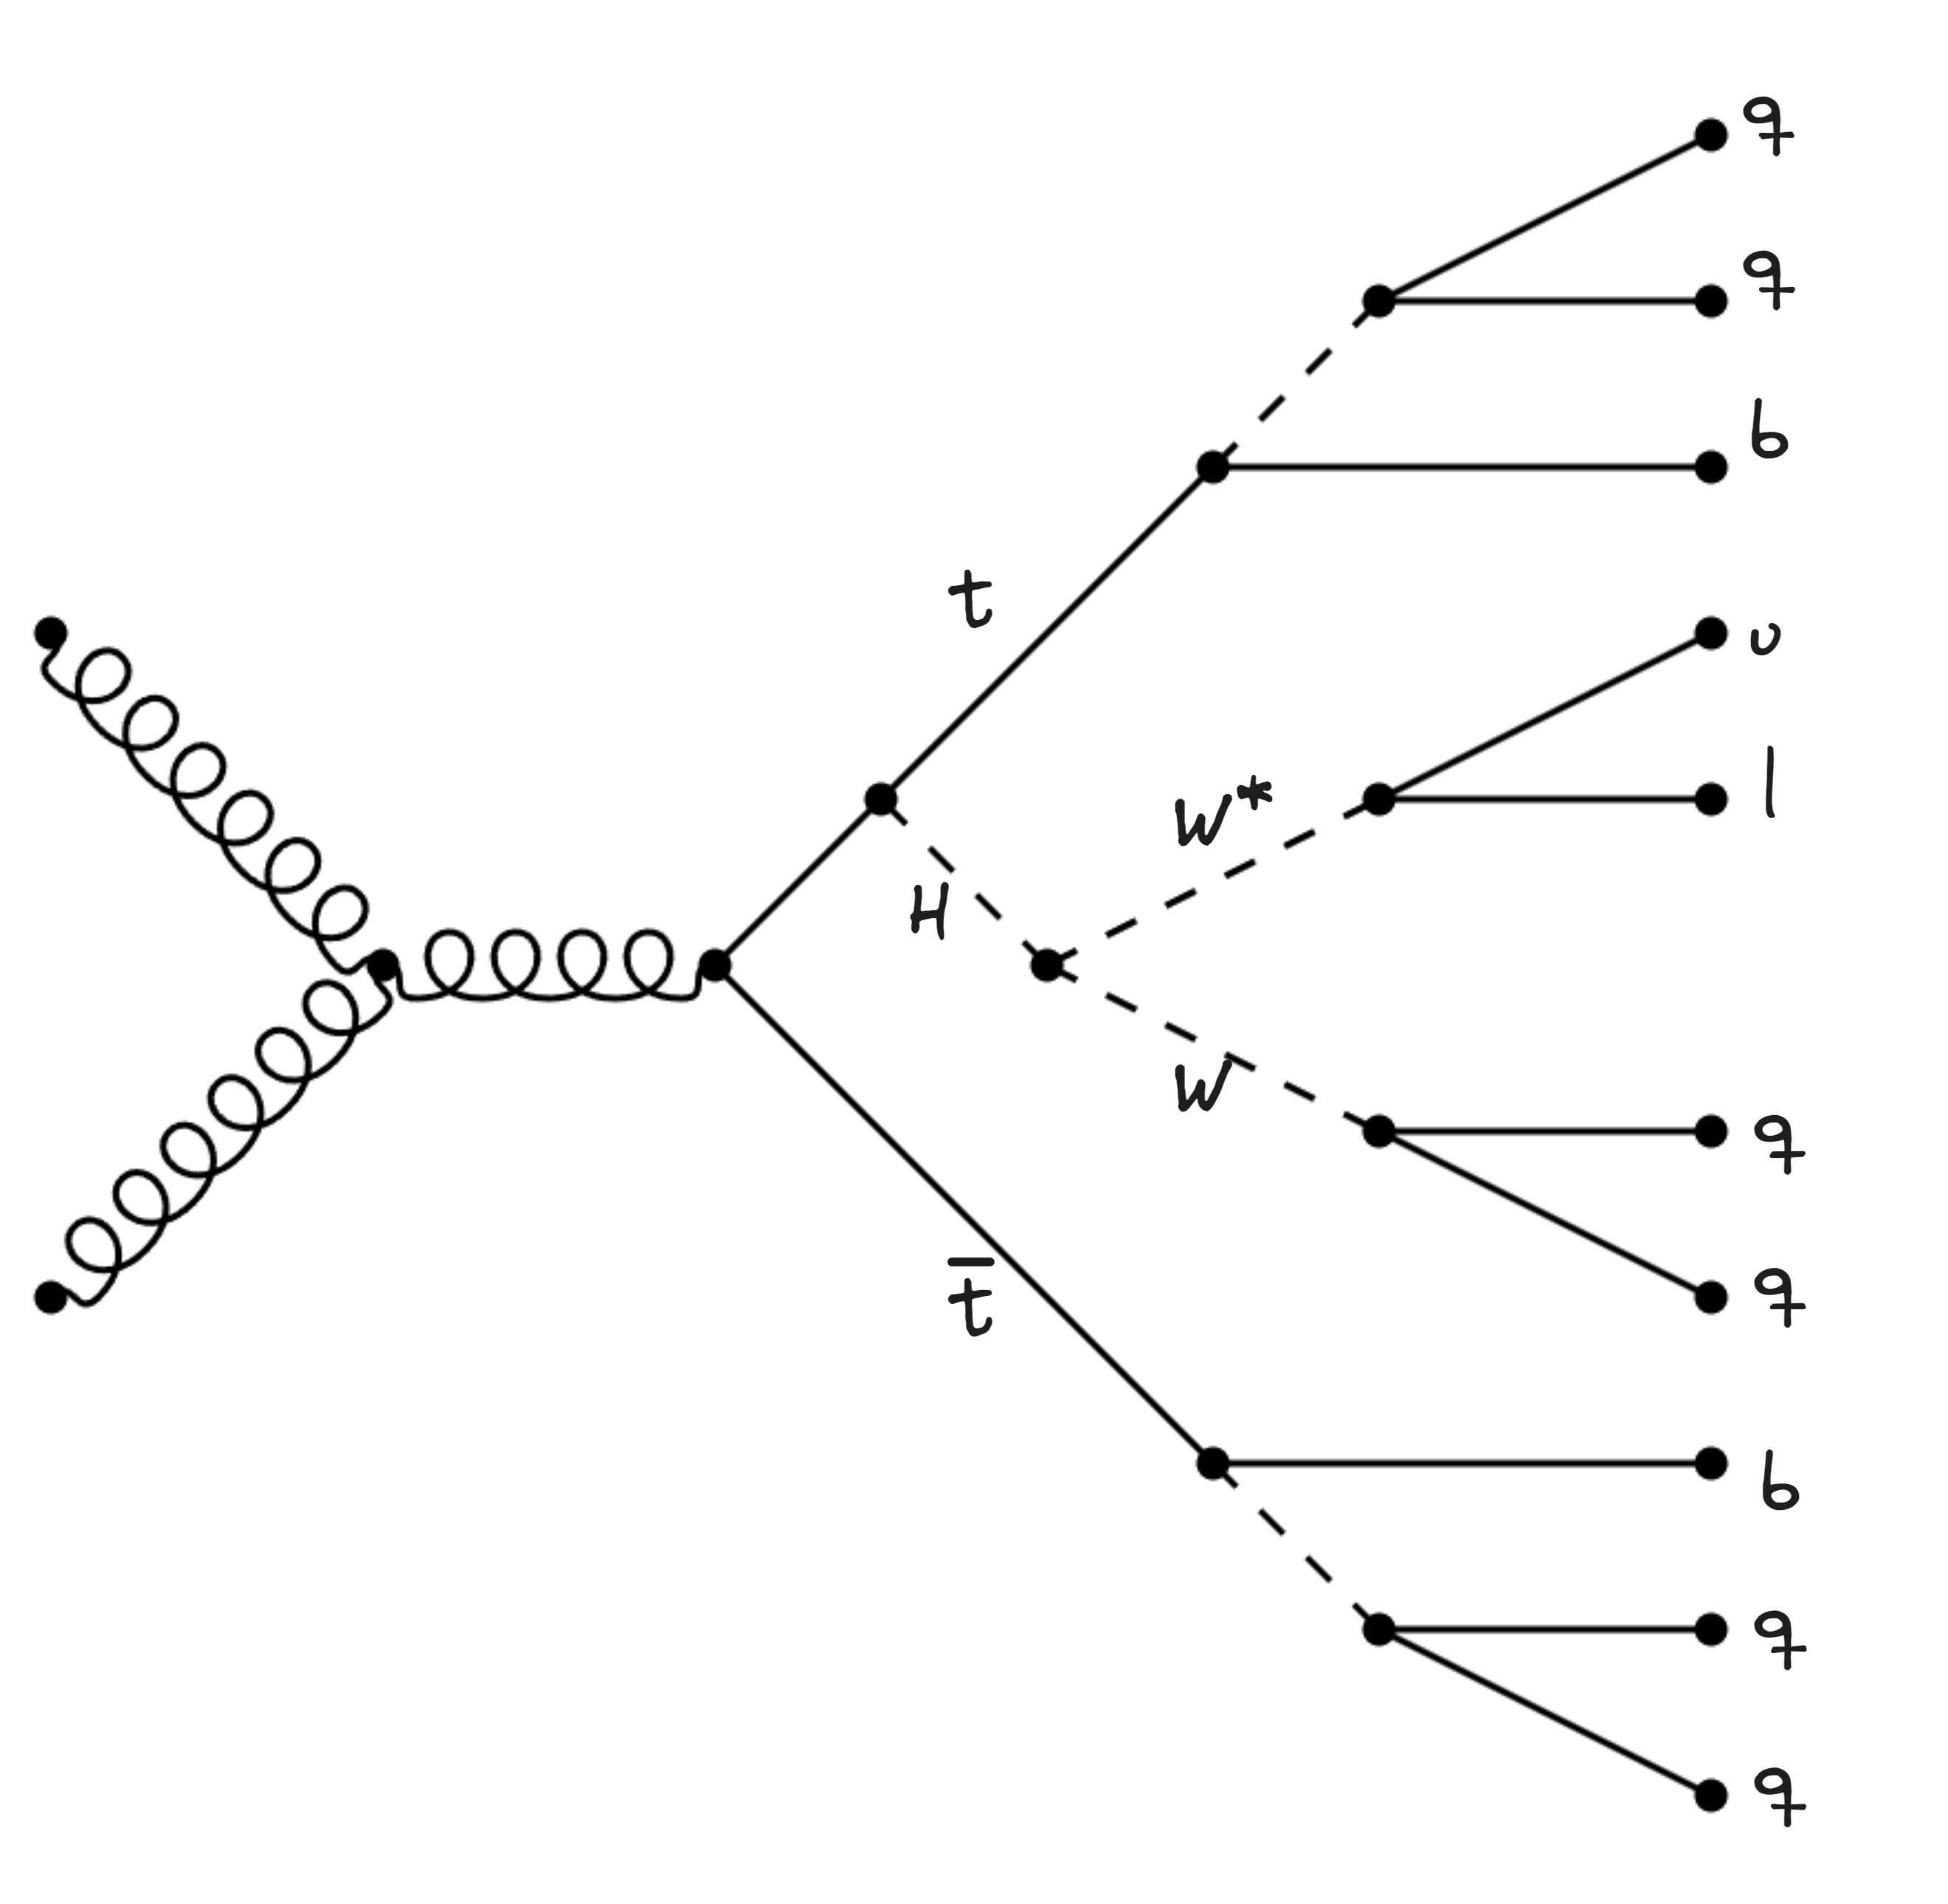
\includegraphics[width=\textwidth]{feynman_diagrams/tthww_undivided.excalidraw.png}
		\end{figure}
	\end{minipage}
\end{frame}

\begin{frame}{Event Topology}{Challenges of the Target Topology}
	\begin{minipage}{.58\textwidth}
		\begin{itemize}
			\item challenges
			\begin{itemize}
				\item 8 quarks to reconstruct
				\item undetected $\nu$ in final state
				\item off-shell mass of $W^*$ from $H$
				\item significant backgrounds
				\begin{itemize}
					\item \ttbarZ and \ttbarW
					\item $t\bar{t}t\bar{t}$
					\item \ttbar + jets (suppressed)
					\item $W$ + jets (suppressed)
				\end{itemize}
			\end{itemize}
			\item assumptions
			\begin{itemize}
				\item SM mass $H$ and on-shell $W$
				\item on-shell hadronic $W\rightarrow qq'$
				\begin{itemize}
					\item further suppress background
					\item improve \spanet training
					\item off-shell leptonic $W^*\rightarrow l\nu$
				\end{itemize}
			\end{itemize}
		\end{itemize}
	\end{minipage}
	\begin{minipage}{.4\textwidth}
		\begin{figure}
			\centering
			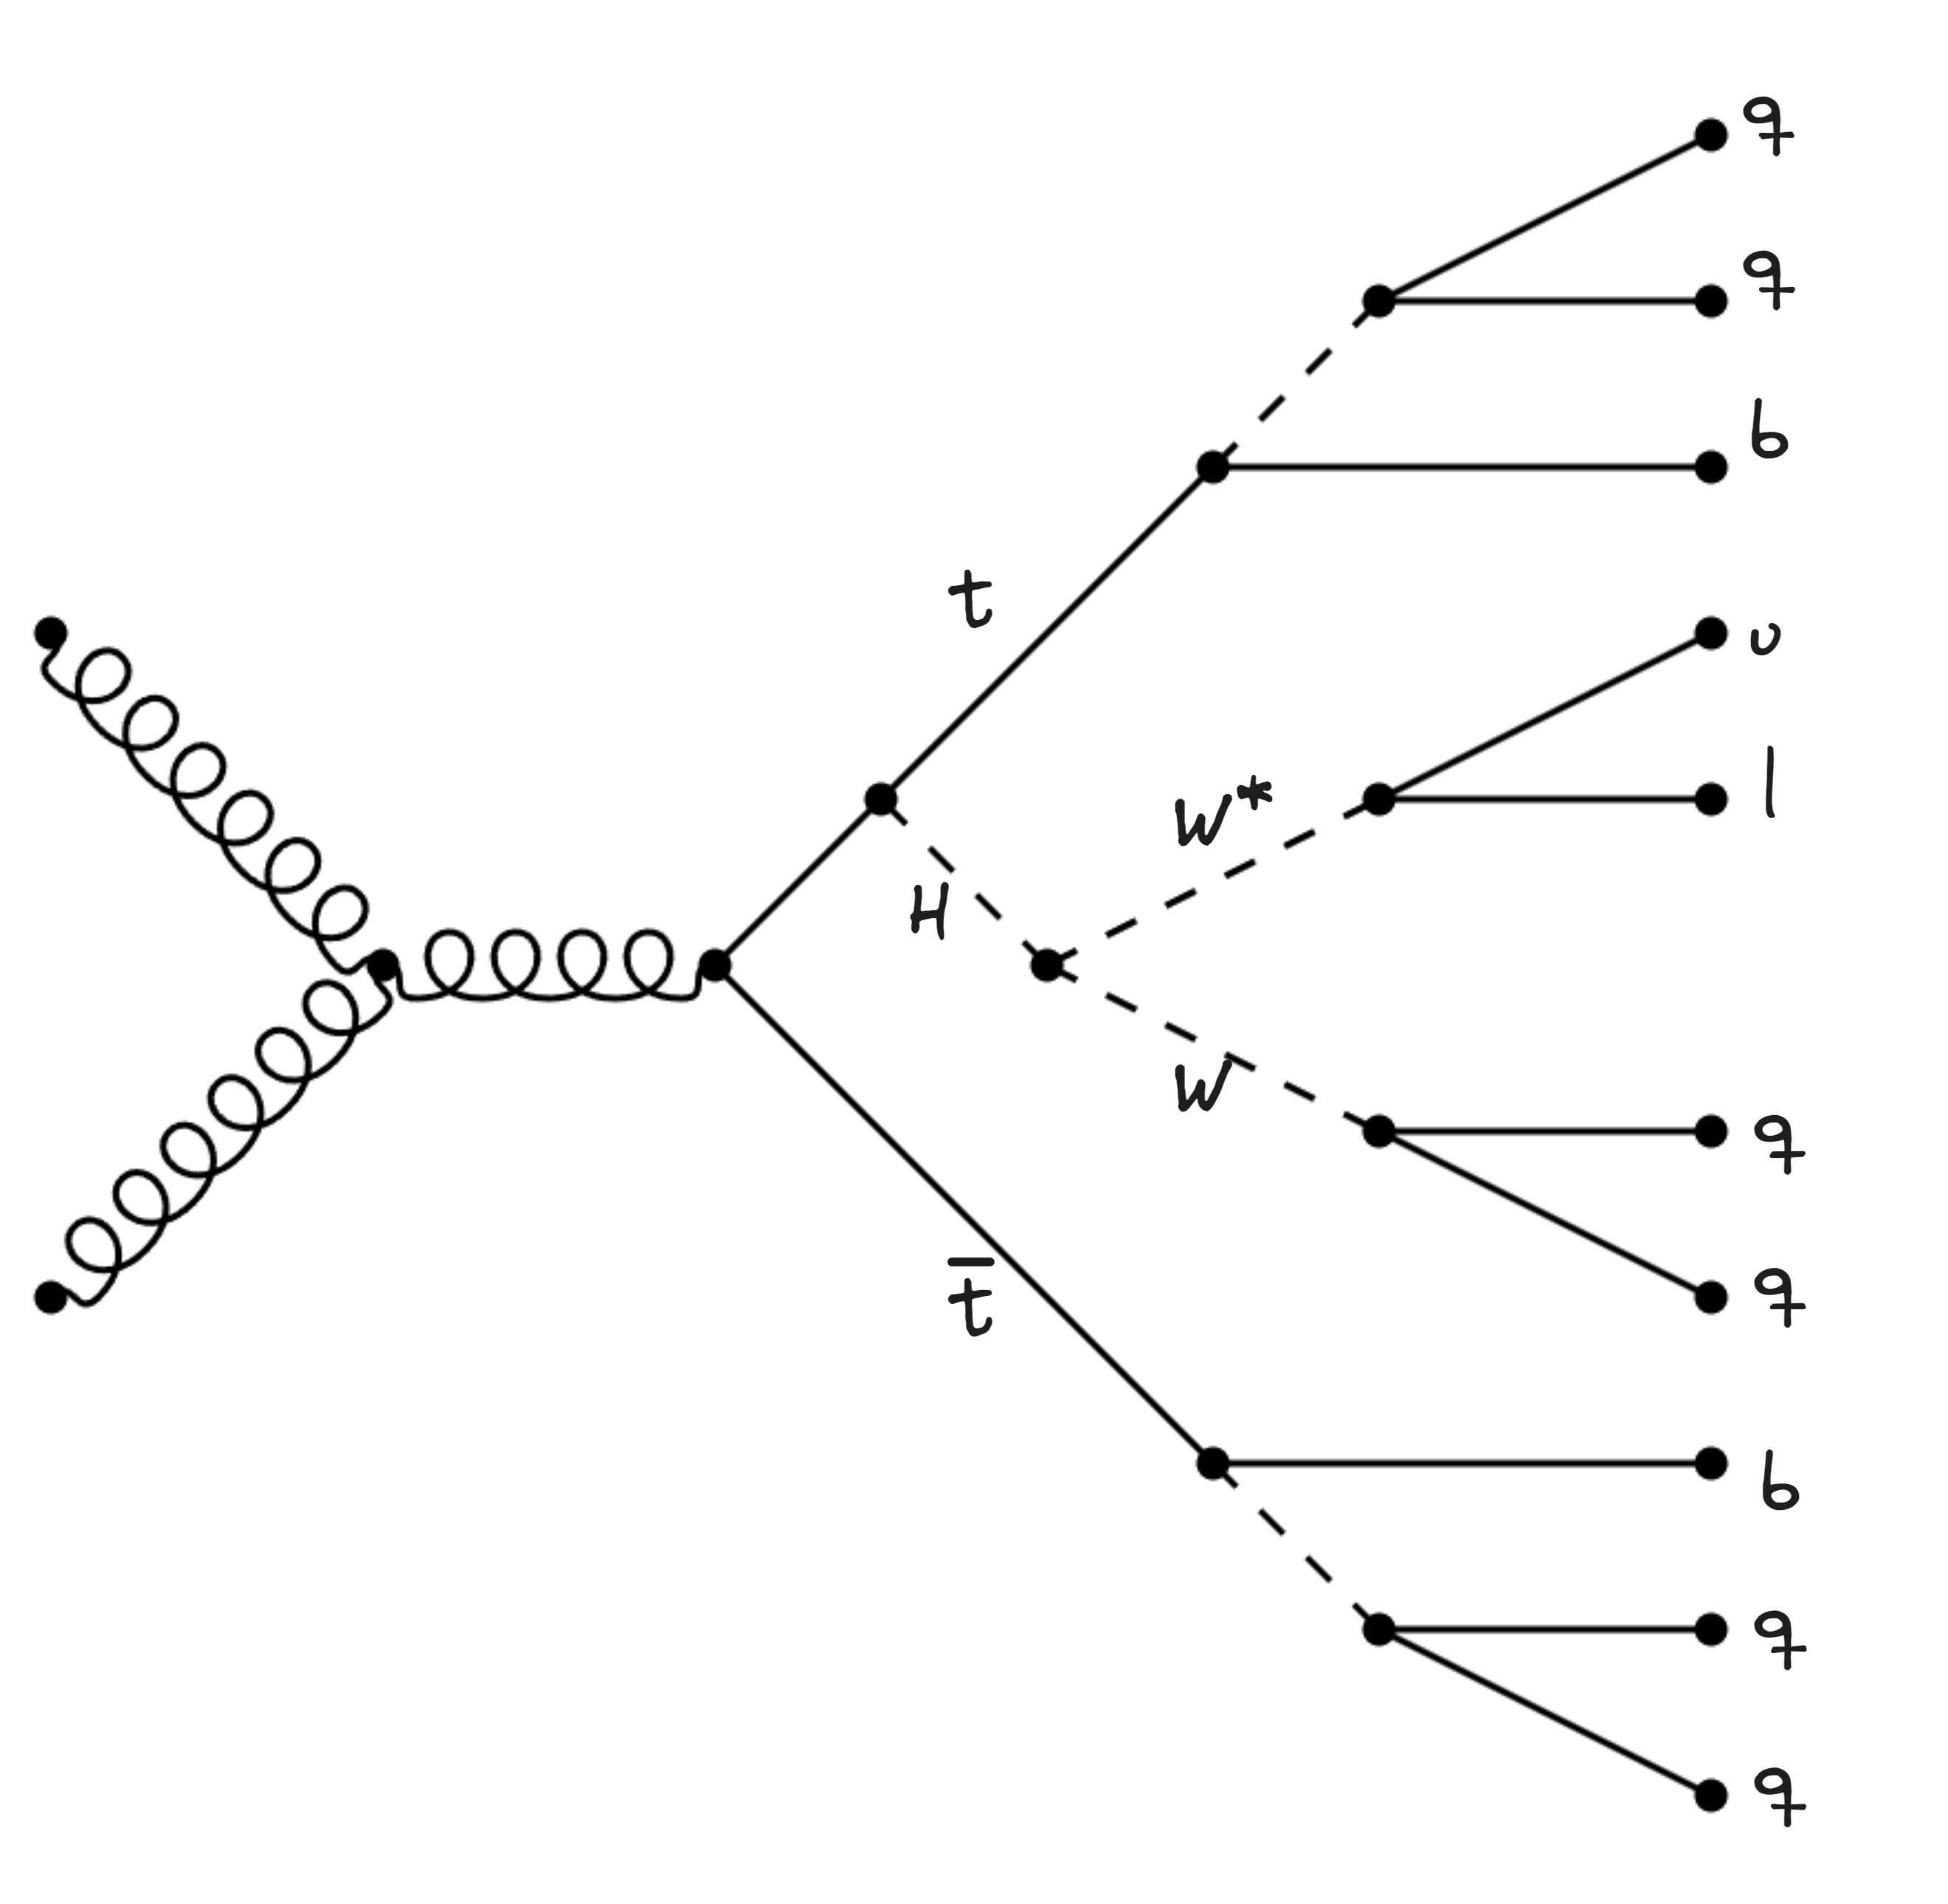
\includegraphics[width=\textwidth]{feynman_diagrams/tthww_undivided.excalidraw.png}
		\end{figure}
	\end{minipage}
\end{frame}

\begin{frame}{Event Topology}{One Step at a Time}
	\begin{minipage}{.58\textwidth}
		\begin{itemize}
			\item subdivide reconstruction task
			\item hadronic (blue): \ttbar and $W_\text{had.}$
			\begin{itemize}
				\item jet-patron assignment problem
				\item \spanet instead of $\chi^2$ (KL-Fitter)
			\end{itemize}
			\item leptonic (red): $W^*_\text{lep.}$
			\begin{itemize}
				\item unknown parameters $\eta_\nu$ and $m_{W^*}$ 
				\item underconstrained system $\Rightarrow$ sample parameters 
				\item neutrino weighting
			\end{itemize}
		\end{itemize}
	\end{minipage}
	\begin{minipage}{.4\textwidth}
		\begin{figure}
			\centering
			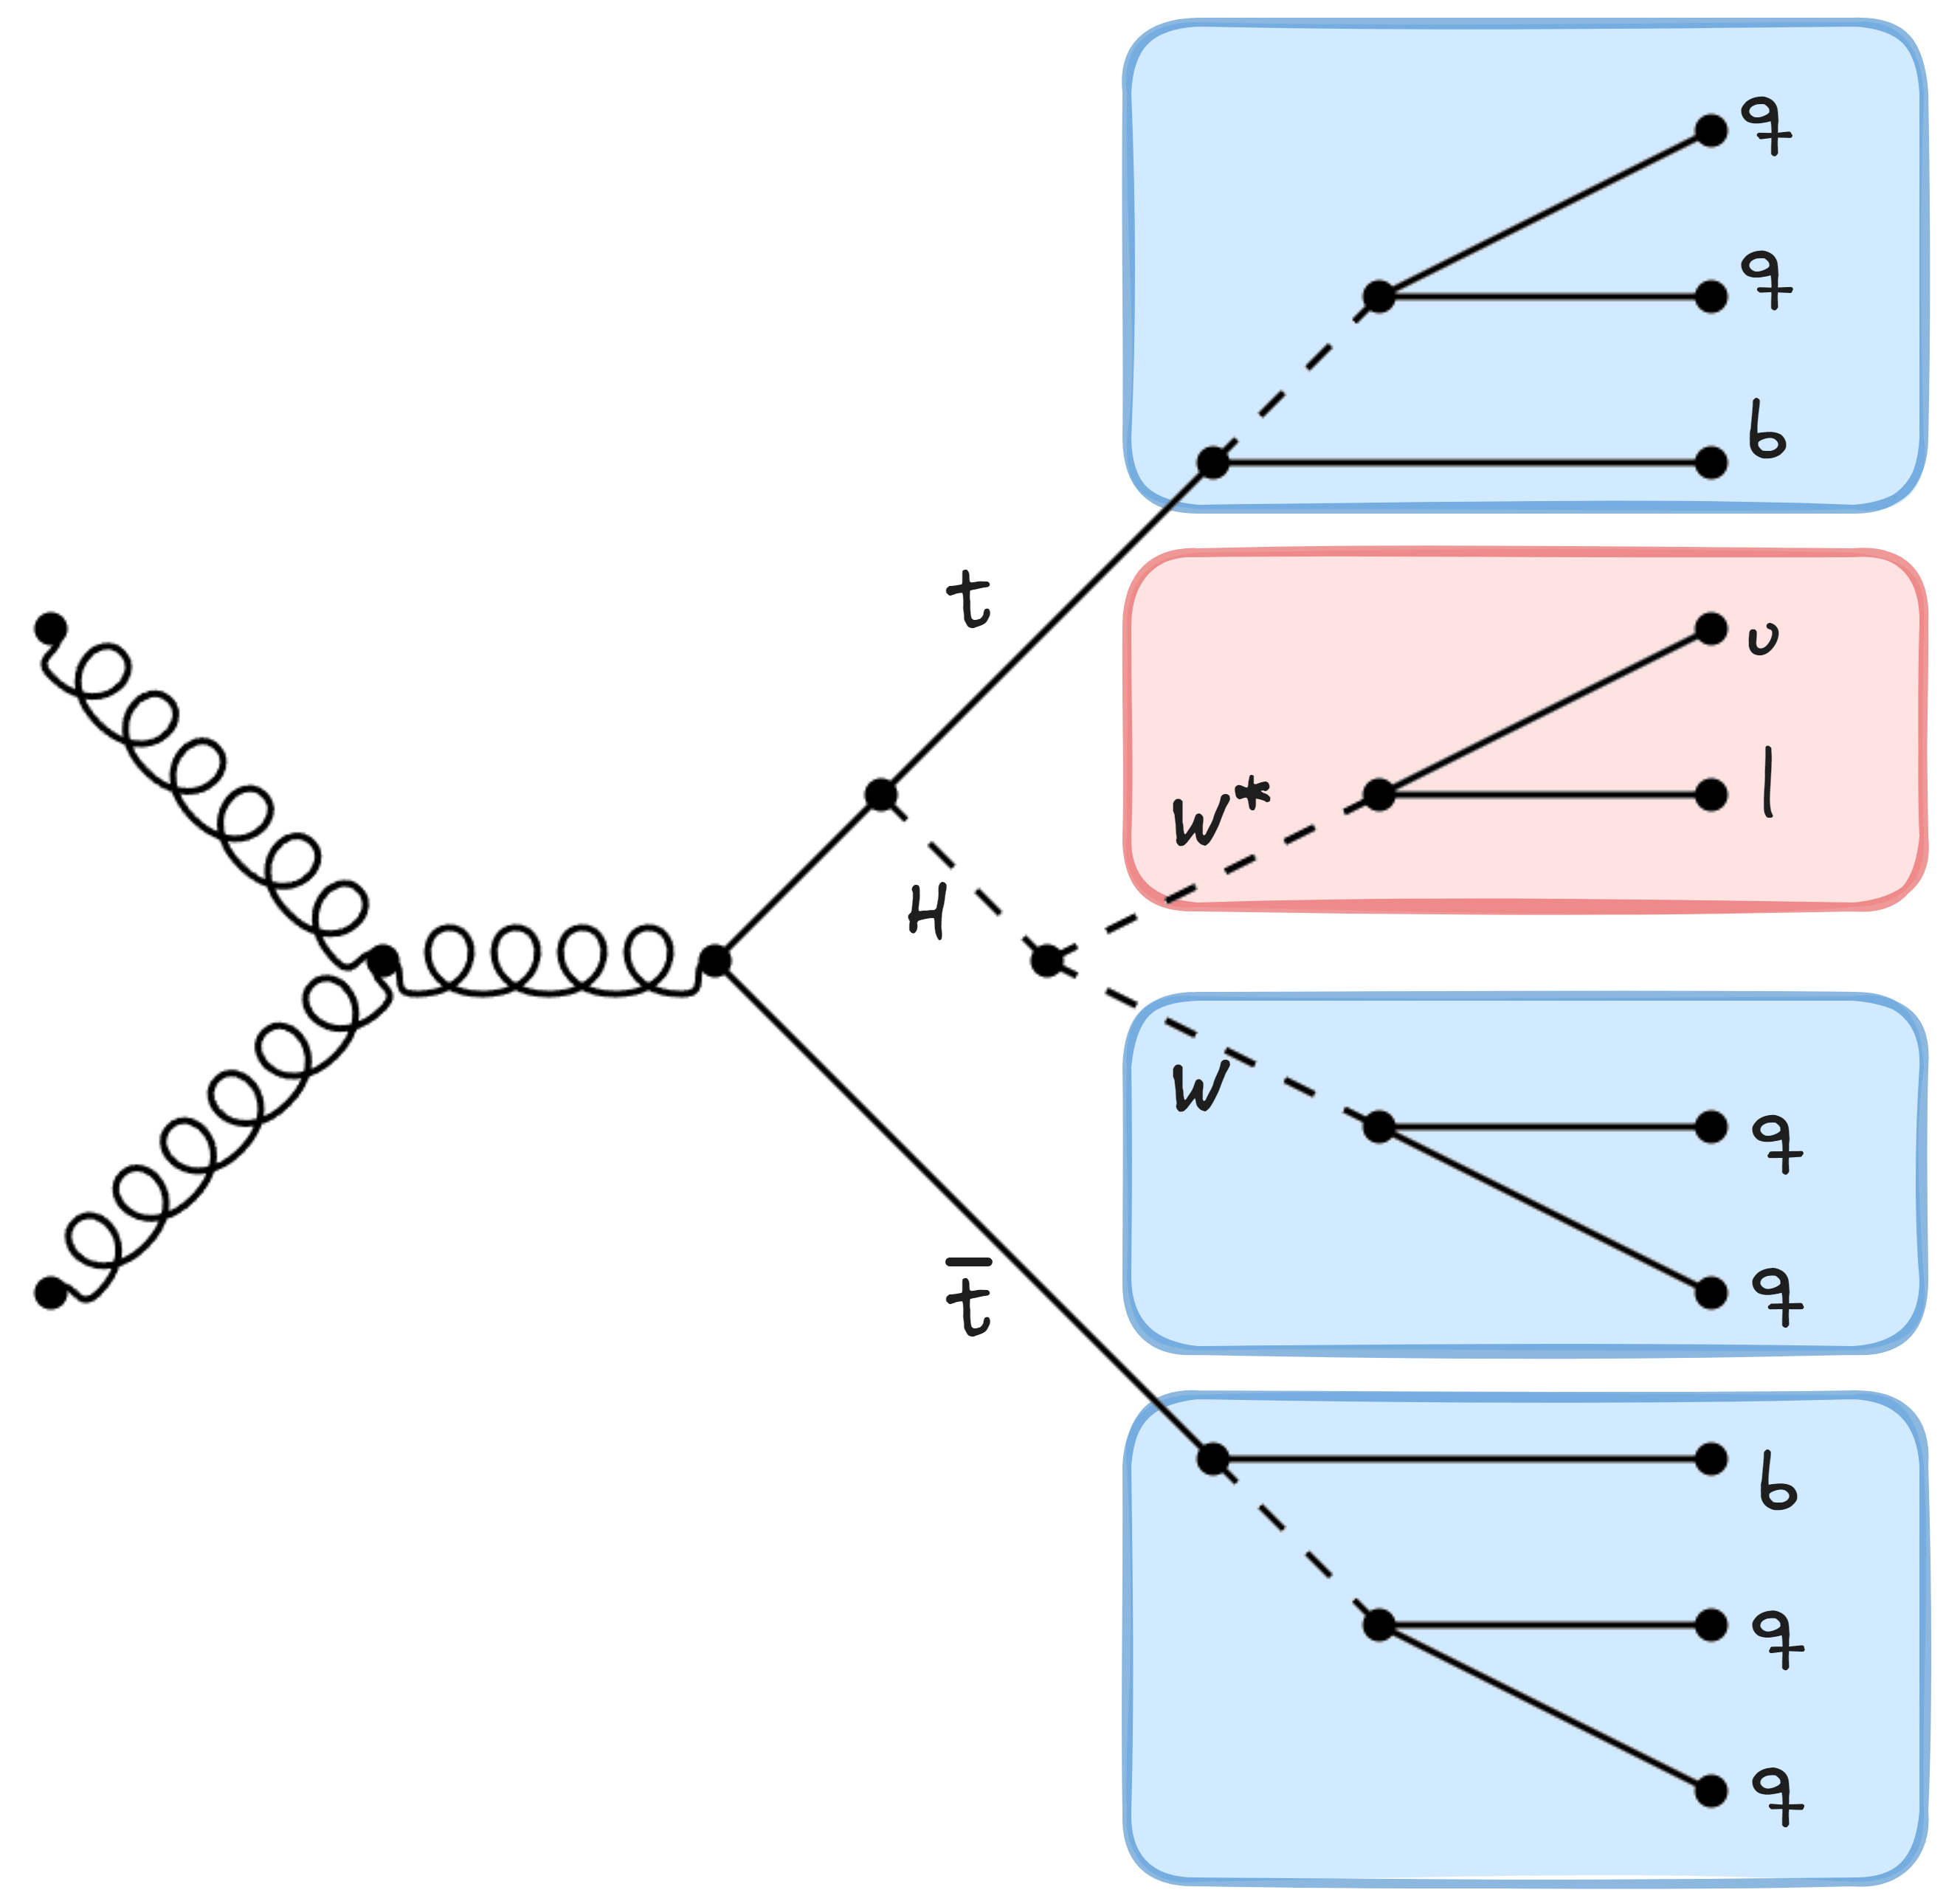
\includegraphics[width=\textwidth]{feynman_diagrams/tthww_divided_f.excalidraw.png}
		\end{figure}
	\end{minipage}
\end{frame}

\begin{frame}{$\chi^2$ Minimisation}{The Classical Approach}
	\begin{minipage}{.58\textwidth}
		\begin{itemize}
			\item final state partons hadronise 
			\begin{itemize}
				\item jet-parton assignment problem
			\end{itemize}
			\item combinatoric approach
			\begin{itemize}
				\item combine jets for reconstructed mass $M$
				\item compare to parton SM mass $m$
				\item sum over all resonances
			\end{itemize}
		\end{itemize}

		\begin{align*}
			\chi^2 = \sum_{i,j} \frac{(M_{q_i}-m_j)^2}{\sigma_j^2}
		\end{align*}

		\begin{itemize}
			\item every possible jet permutation tested $\Rightarrow$ slow
			\item reducing permutation using tagging
			\begin{itemize}
				\item mis-tags $\Rightarrow$ impossible reconstructions 
			\end{itemize} 
		\end{itemize}
	  \end{minipage}\hfill
	  \begin{minipage}{.4\textwidth}
		  \begin{figure}
			  \centering
			  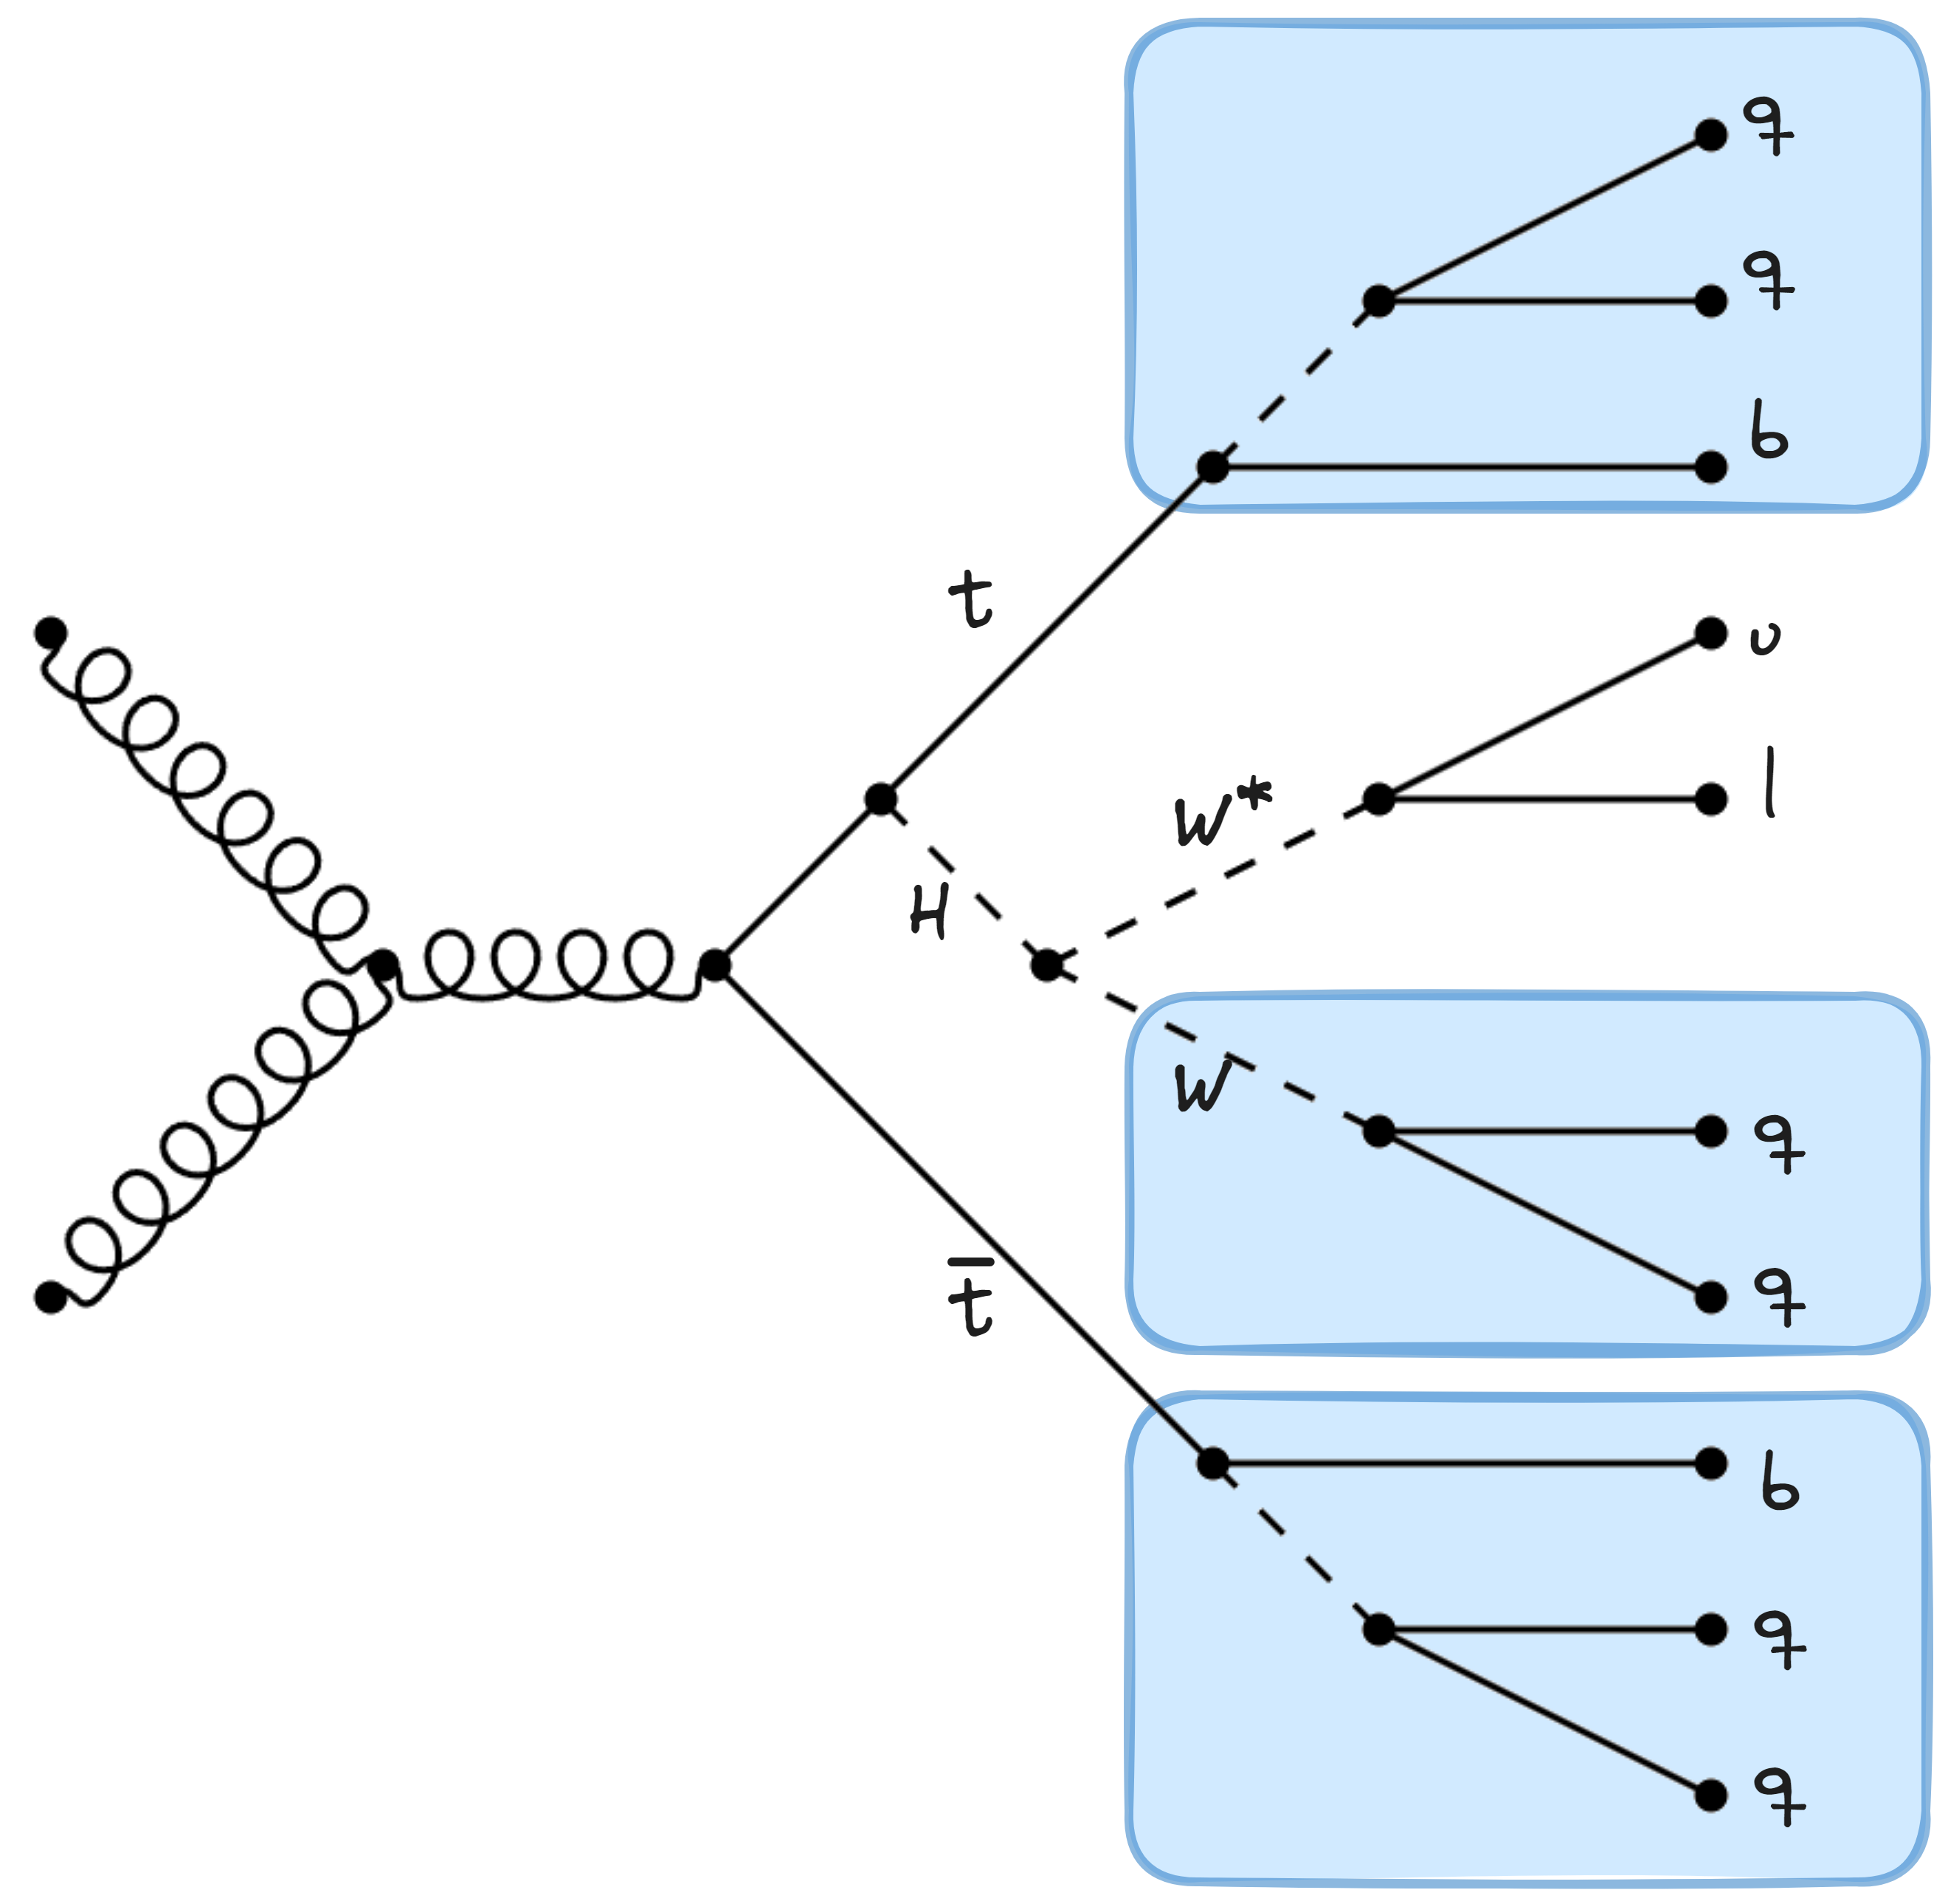
\includegraphics[width=\textwidth]{feynman_diagrams/tthww_divided_d.excalidraw.png}	
		  \end{figure}
	  \end{minipage}
\end{frame}

\begin{frame}{SPA-Net}{The Modern Approach}
	\begin{minipage}{.58\textwidth}
		\begin{itemize}
			\item \spanet (Symmetry Preserving Attention Networks)
			\begin{itemize}
				\item input: jets, $b$-tags, leptons, event info
				\item output: jet-parton assignment
			\end{itemize}
			\item properties of \spanet
			\begin{itemize}
				\item agnostic to number of input objects
				\item unique parton assignment
				\item symmetries from laws of physics 
				\item training needs truth matched inputs
			\end{itemize}
			\item symmetries
			\begin{itemize}
				\item reduction of possible jet permutation $\Rightarrow$ fast
				\item particle symmetry (jet origin $q\leftrightarrow \bar{q}\leftrightarrow g$)
				\item jet symmetry (swap label of decays $q\bar{q}\leftrightarrow\bar{q}q$)
			\end{itemize}
		\end{itemize}
	  \end{minipage}\hfill
	  \begin{minipage}{.4\textwidth}
		  \begin{figure}
			  \centering
			  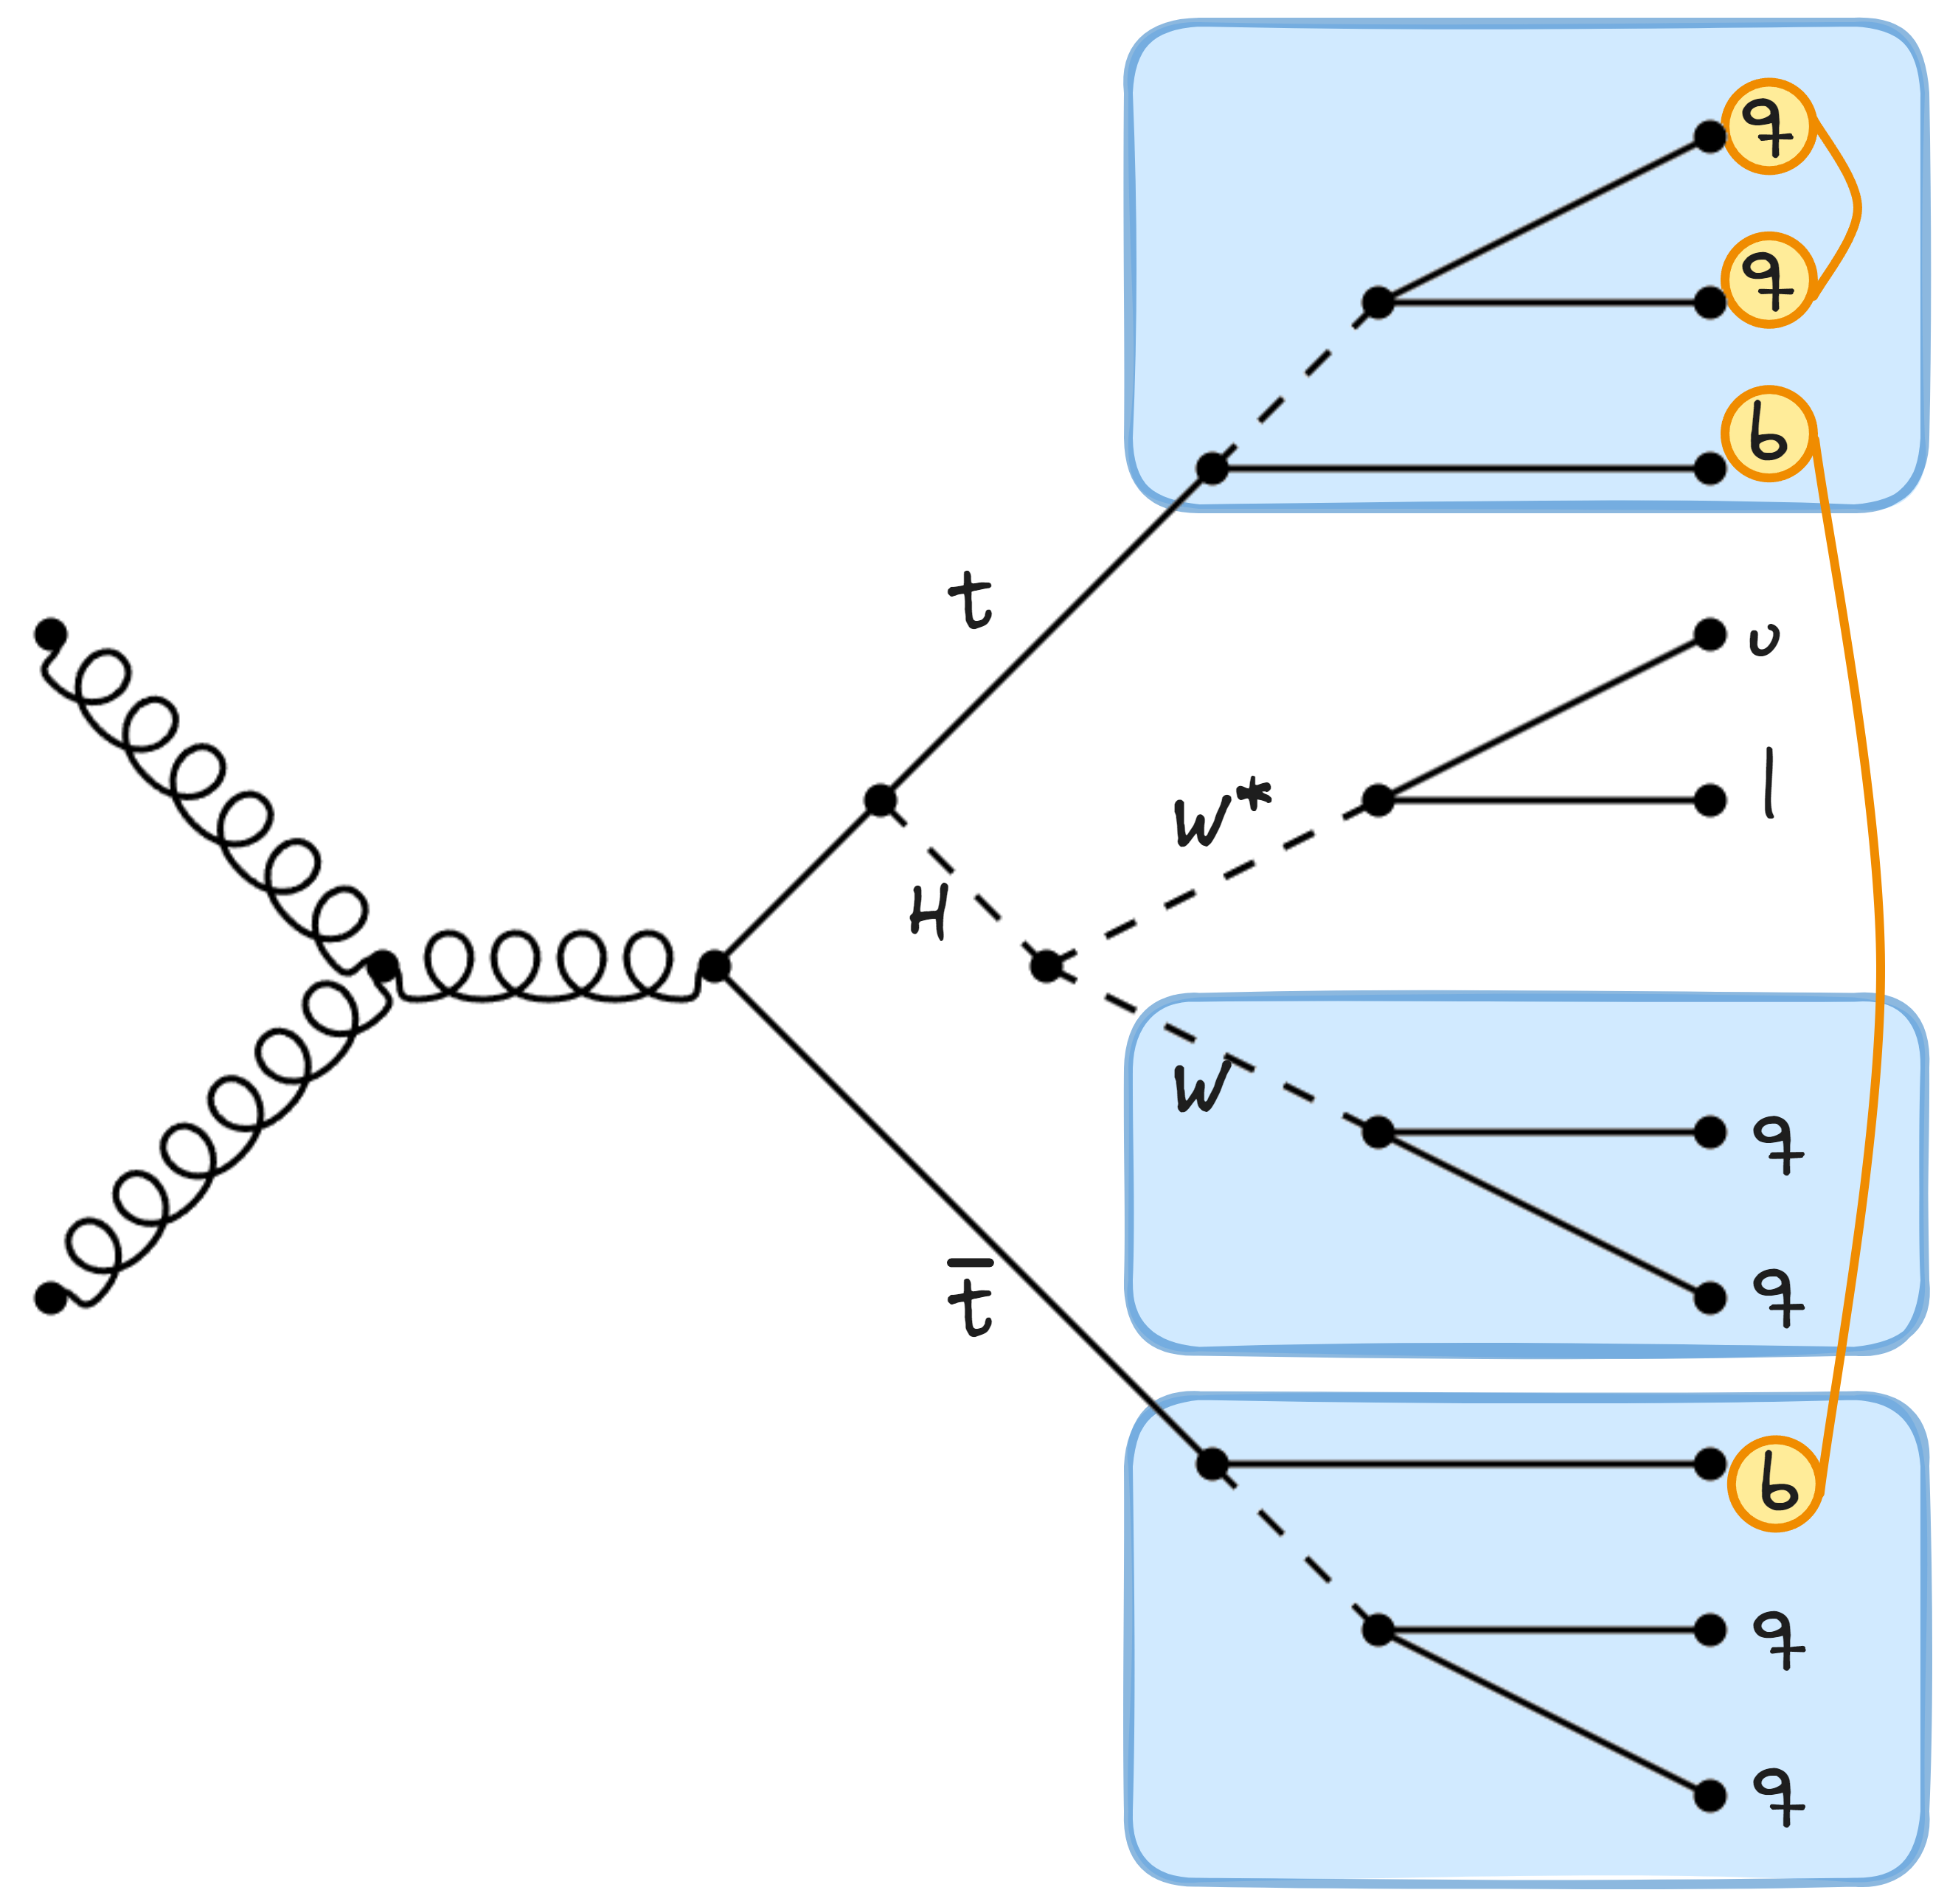
\includegraphics[width=\textwidth]{feynman_diagrams/tthww_divided_g.excalidraw.png}	
		  \end{figure}
	  \end{minipage}
\end{frame}

\begin{frame}{SPA-Net}{Under the Hood}
    % \begin{itemize}
	% 	\item high-level overview
	% 	\begin{itemize}
	% 		\item embeddings $\Rightarrow$ latent space representation for each input object
	% 		\item central transformer $\Rightarrow$ combined for all
	% 		\item particle transformer $\Rightarrow$ separated for each resonance particle
	% 		\item tensor-attention $\Rightarrow$ jet-parton assignment incl. confidence 
	% 	\end{itemize}
	% \end{itemize}
  
	\begin{figure}
		\centering
		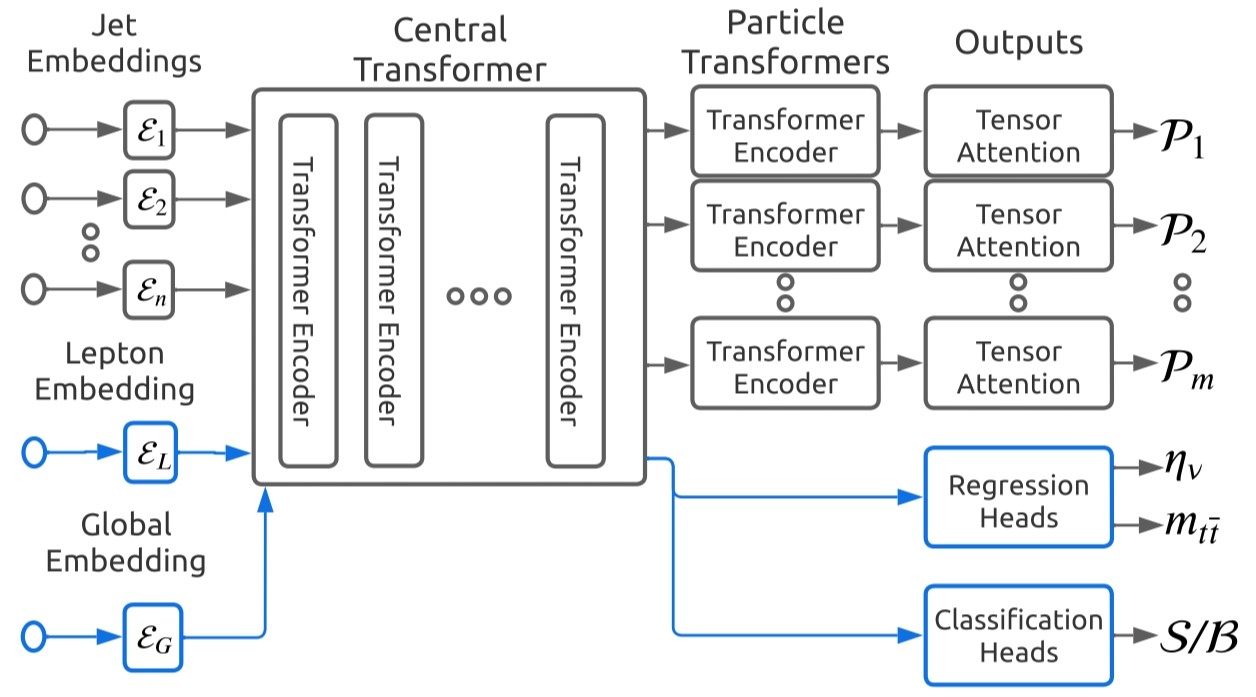
\includegraphics[width=.65\textwidth]{methods/spanet_architecture_2.jpg}
		
		% \vspace{-4mm}{\tiny figure taken from SciPost Phys. 12, 178(2022)}
	\end{figure}
\end{frame}

\begin{frame}{SPA-Net}{Workflow}
	\begin{minipage}{.58\textwidth}
		\begin{itemize}
			\item first step of the reconstruction
			\item needs MC training samples
			\item \spanets prediction of jet assignment
			\begin{itemize}
				\item used as input for neutrino weighting
				\item later applied in final reconstruction
			\end{itemize}
		\end{itemize}
	  \end{minipage}\hfill
	  \begin{minipage}{.2\textwidth}
		  \begin{figure}
			  \centering
			  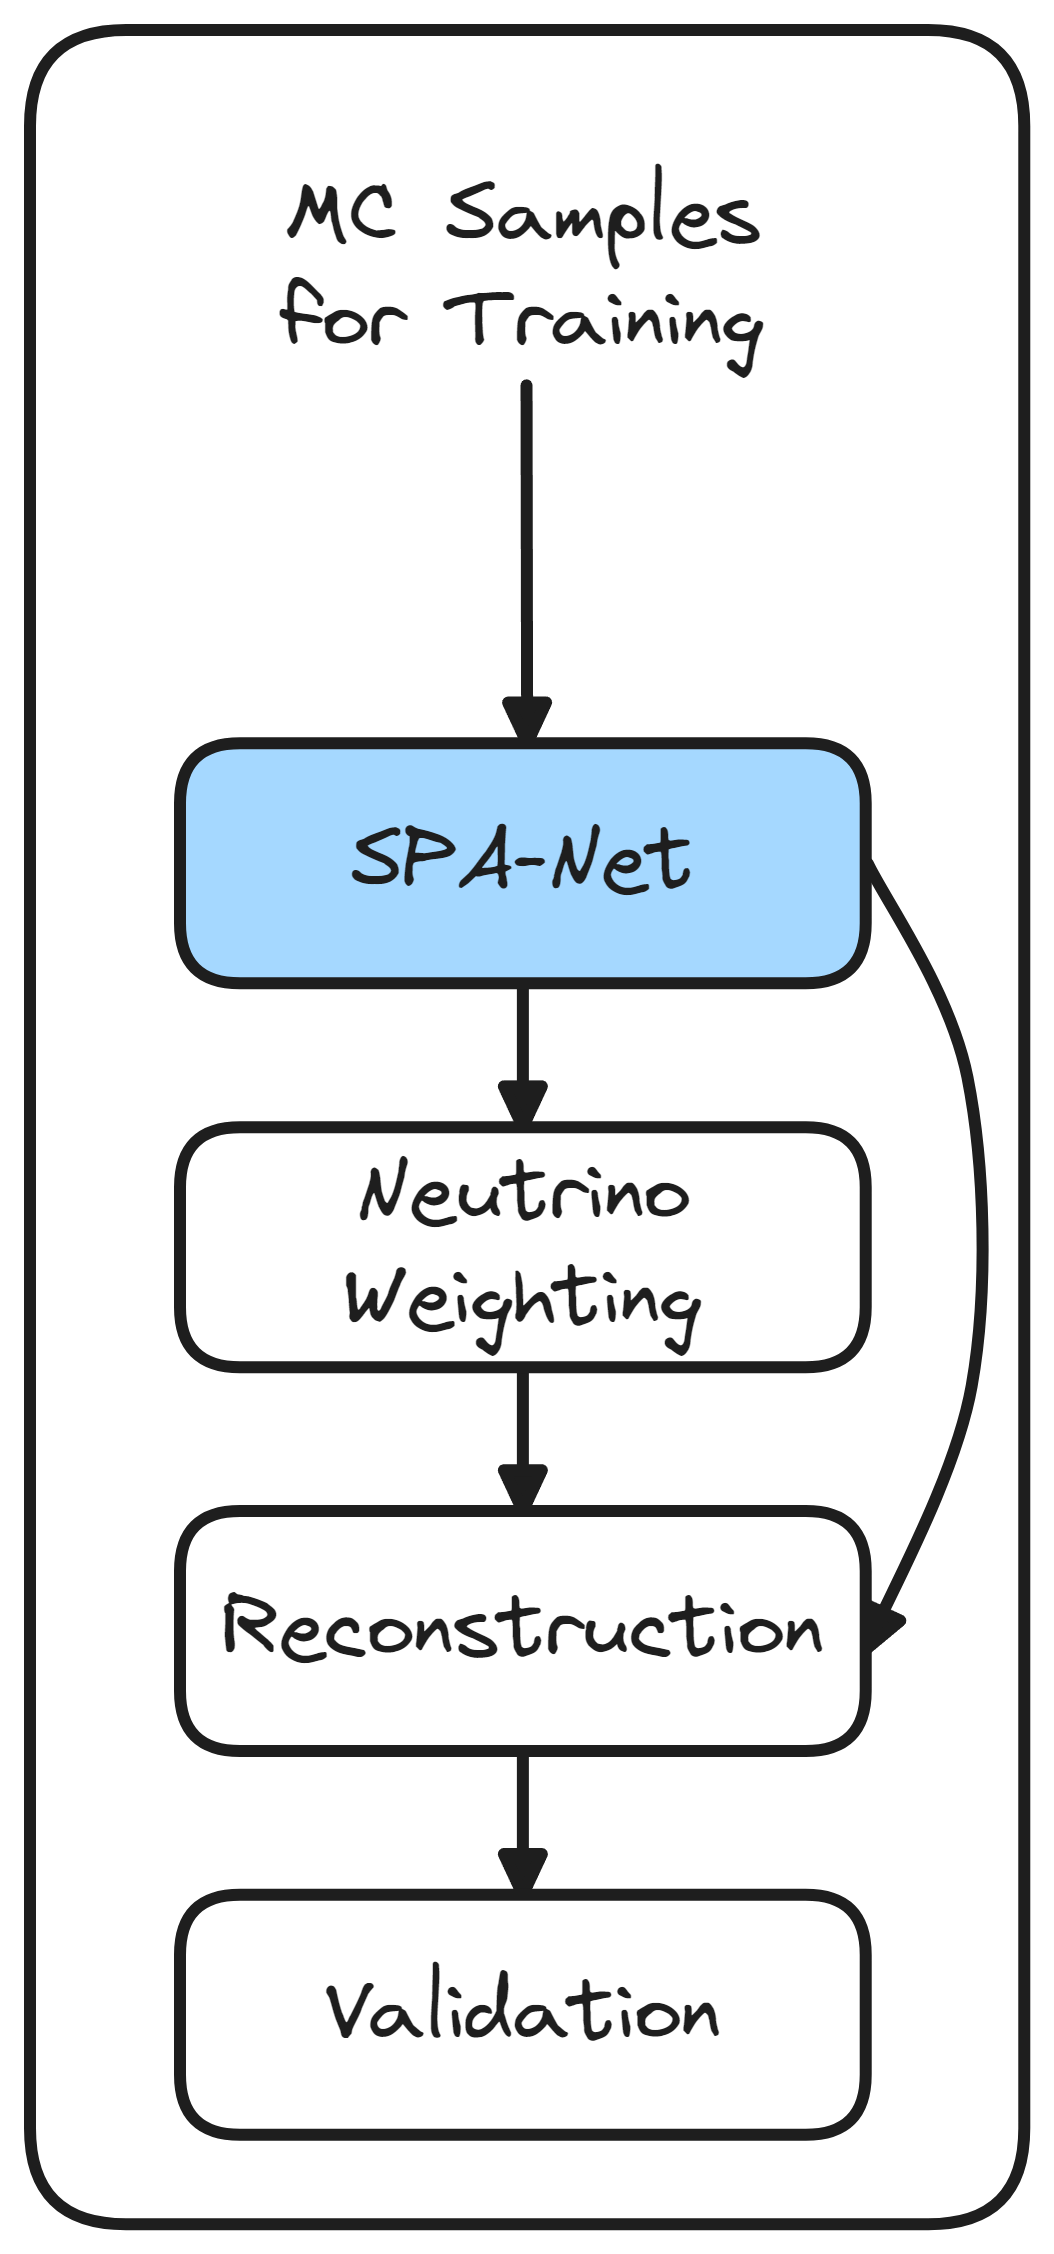
\includegraphics[width=\textwidth]{flowchart/flowchart_c.excalidraw.png}	
		  \end{figure}
	  \end{minipage}
\end{frame}

\begin{frame}{Neutrino Weighting}{Sampling the Unknown}
	\begin{minipage}{.58\textwidth}
		\begin{itemize}
			\item weighting technique
			\begin{itemize}
				\item sample possible (unknown) parameters
				\item compare to observations
				\item calculate likelihood for sample
			\end{itemize}
			\item success in dileptonic \ttbar analysis (@\atlas, \dzero)
			\begin{itemize}
				\item underconstrained system due to 2$\nu$
				\item assume $m_t$ + sample $\eta_{\nu_i}$ 
				\item compare $\sum p_T^{\nu_i}$ $\leftrightarrow$ $E_T^\text{miss}$ $\Rightarrow$ most likely $p_T^{\nu_i}$  
			\end{itemize}
			\item needs adaption for $W^*\rightarrow l\nu$  
			\item background suppression
			\begin{itemize}
				\item use neutrino weight in selection $\Rightarrow$ suppress background
			\end{itemize} 
		\end{itemize}
	\end{minipage}\hfill
	\begin{minipage}{.4\textwidth}
		\begin{figure}
			\centering
			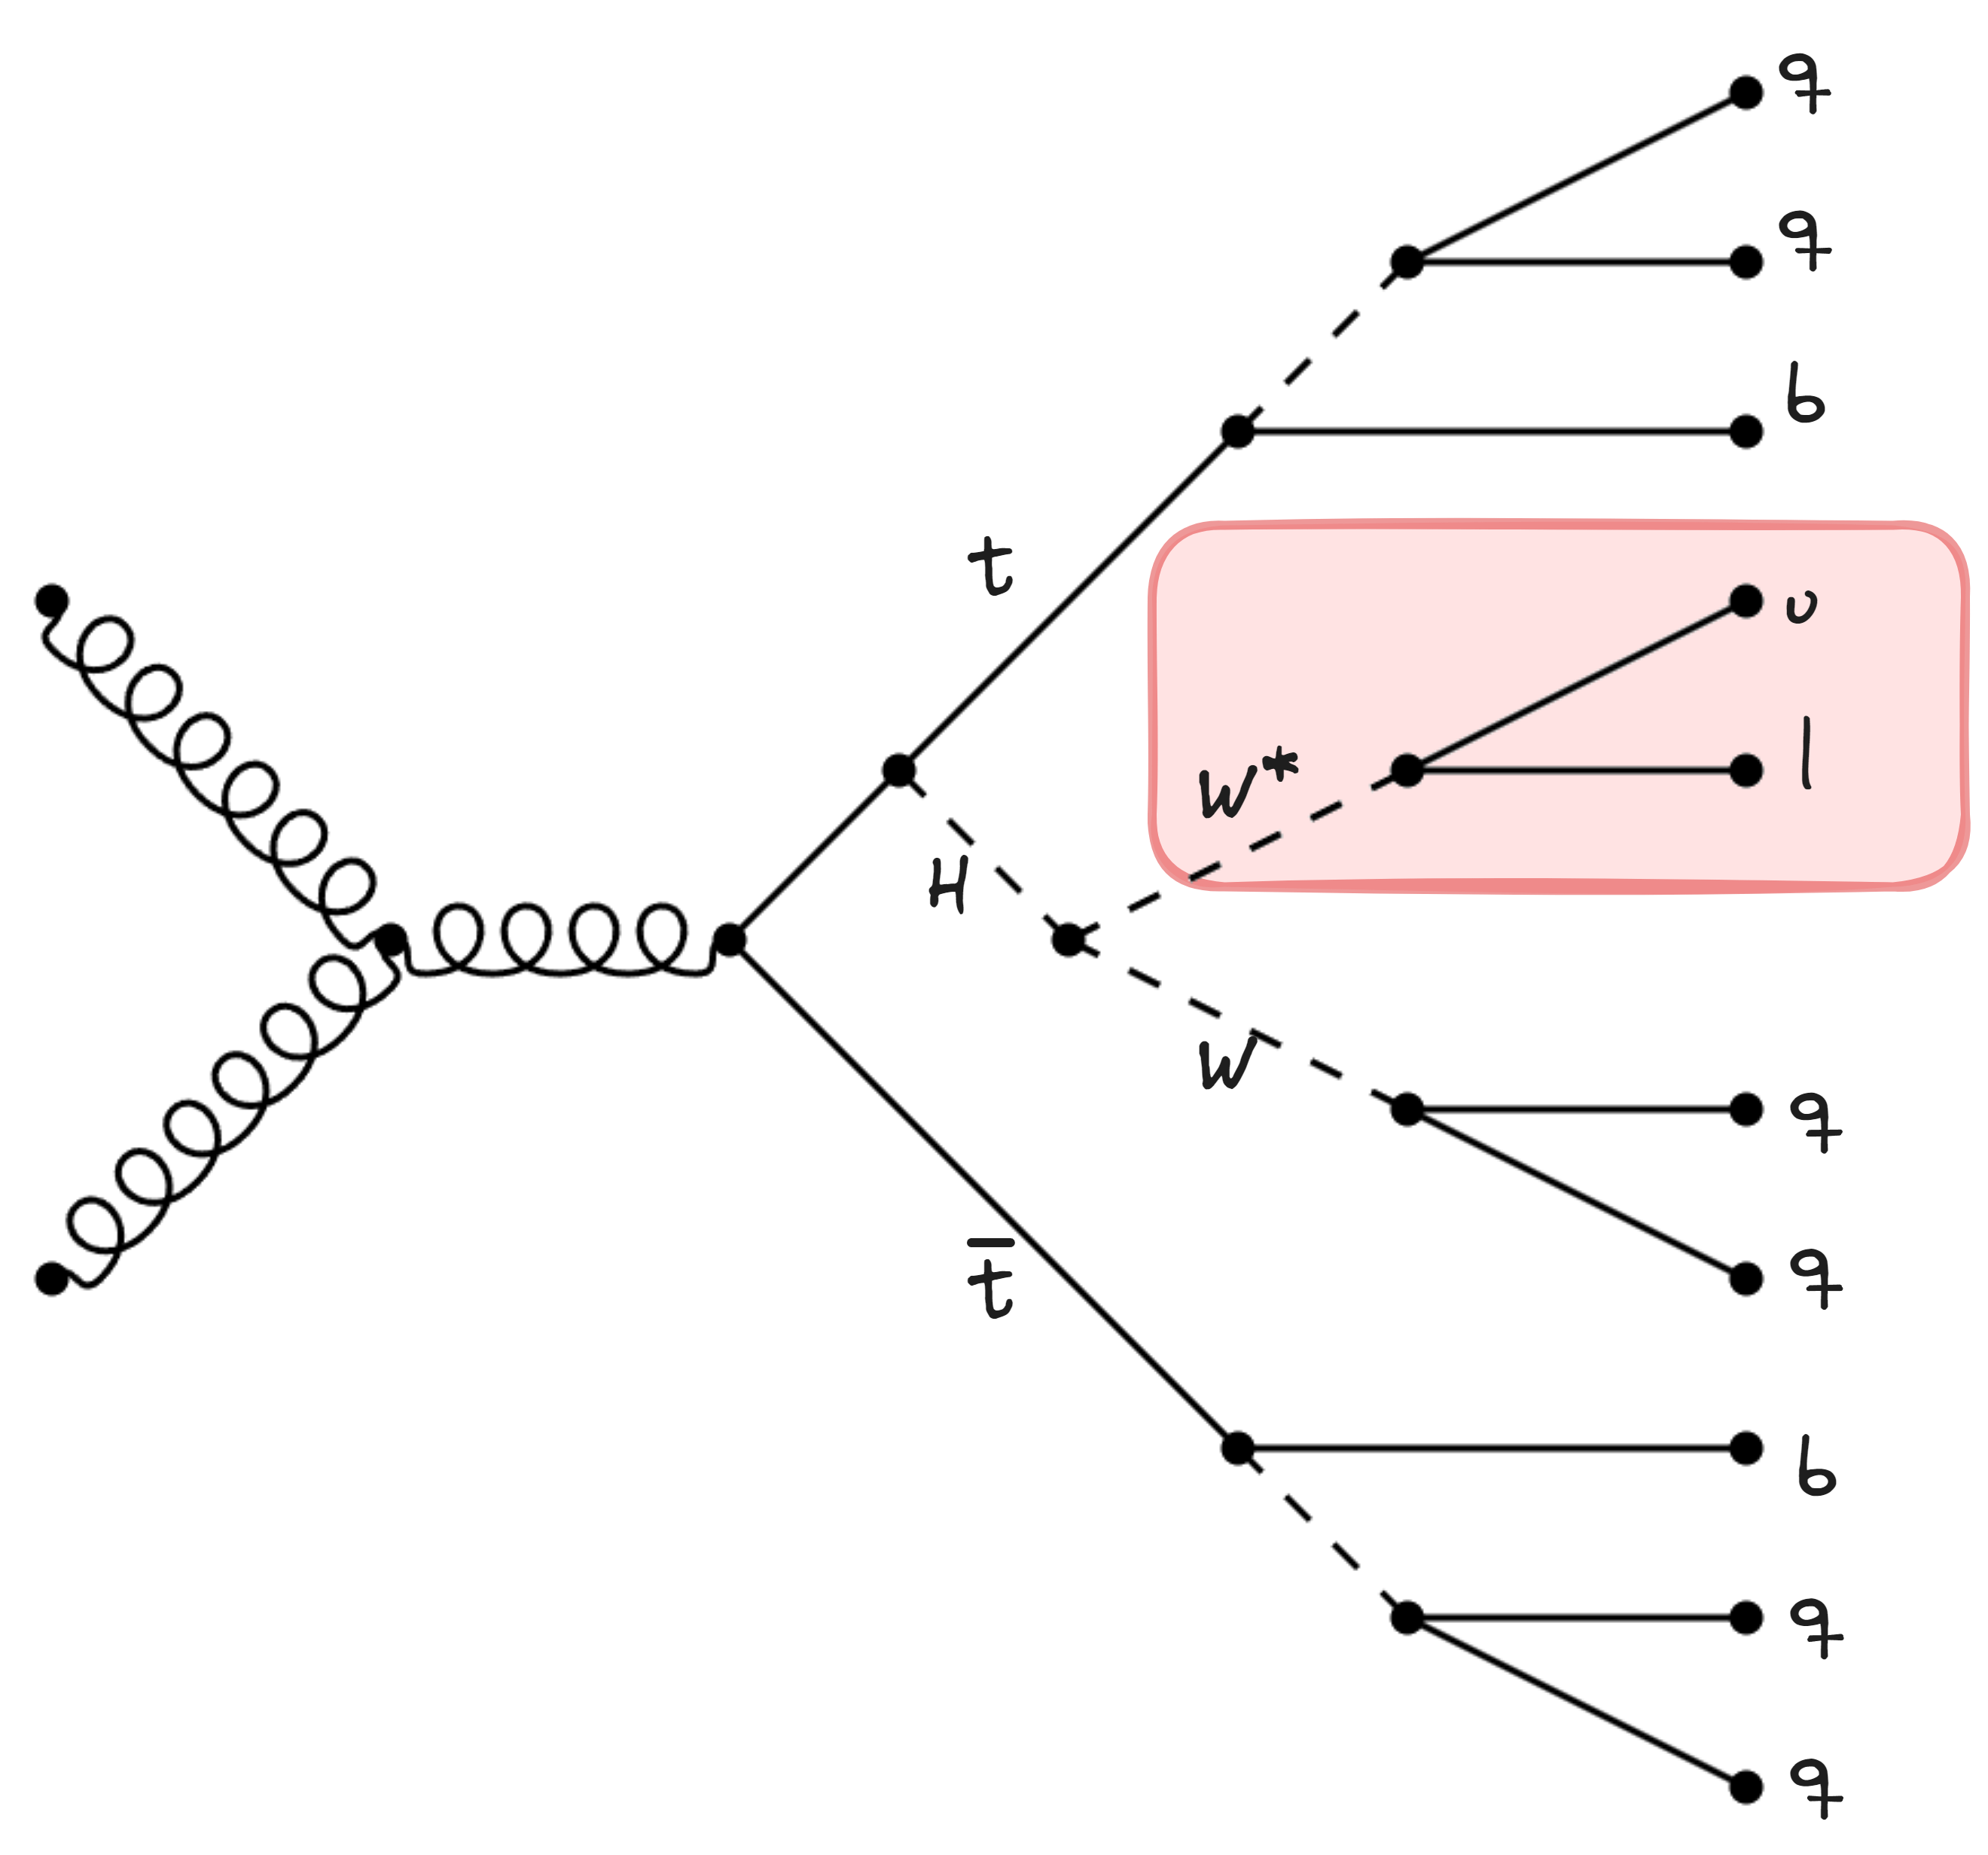
\includegraphics[width=\textwidth]{feynman_diagrams/tthww_divided_e.excalidraw.png}	
		\end{figure}
	\end{minipage}
\end{frame}

\begin{frame}{Neutrino Weighting}{Adaptation}
	\begin{minipage}{.60\textwidth}
		\begin{itemize}
			\item calculate neutrino $p_{x,y}^\nu$ from sampling
			\begin{itemize}
				\item $\nu$ pseudo-rapidity $\eta_\nu$
				\item $W^*$ off-shell mass $m_W$
				\item comparison: $p_{x,y}^\text{miss}$ $\leftrightarrow$ $p_{x,y}^\nu$
			\end{itemize}	
			\item mathematically 0,1 or 2 solutions possible
		\end{itemize}

		\begin{align*}
			w = \exp\left(\frac{(p_x^\nu-p_x^\text{miss})^2}{\sigma_x^2}\right) \cdot \exp\left(\frac{(p_y^\nu-p_y^\text{miss})^2}{\sigma_y^2}\right)
		\end{align*}

		\begin{itemize}
			\item code is available $\Rightarrow$ validation still needed
		\end{itemize}
	\end{minipage}\hfill
	\begin{minipage}{.38\textwidth}
		\begin{figure}
			\centering
			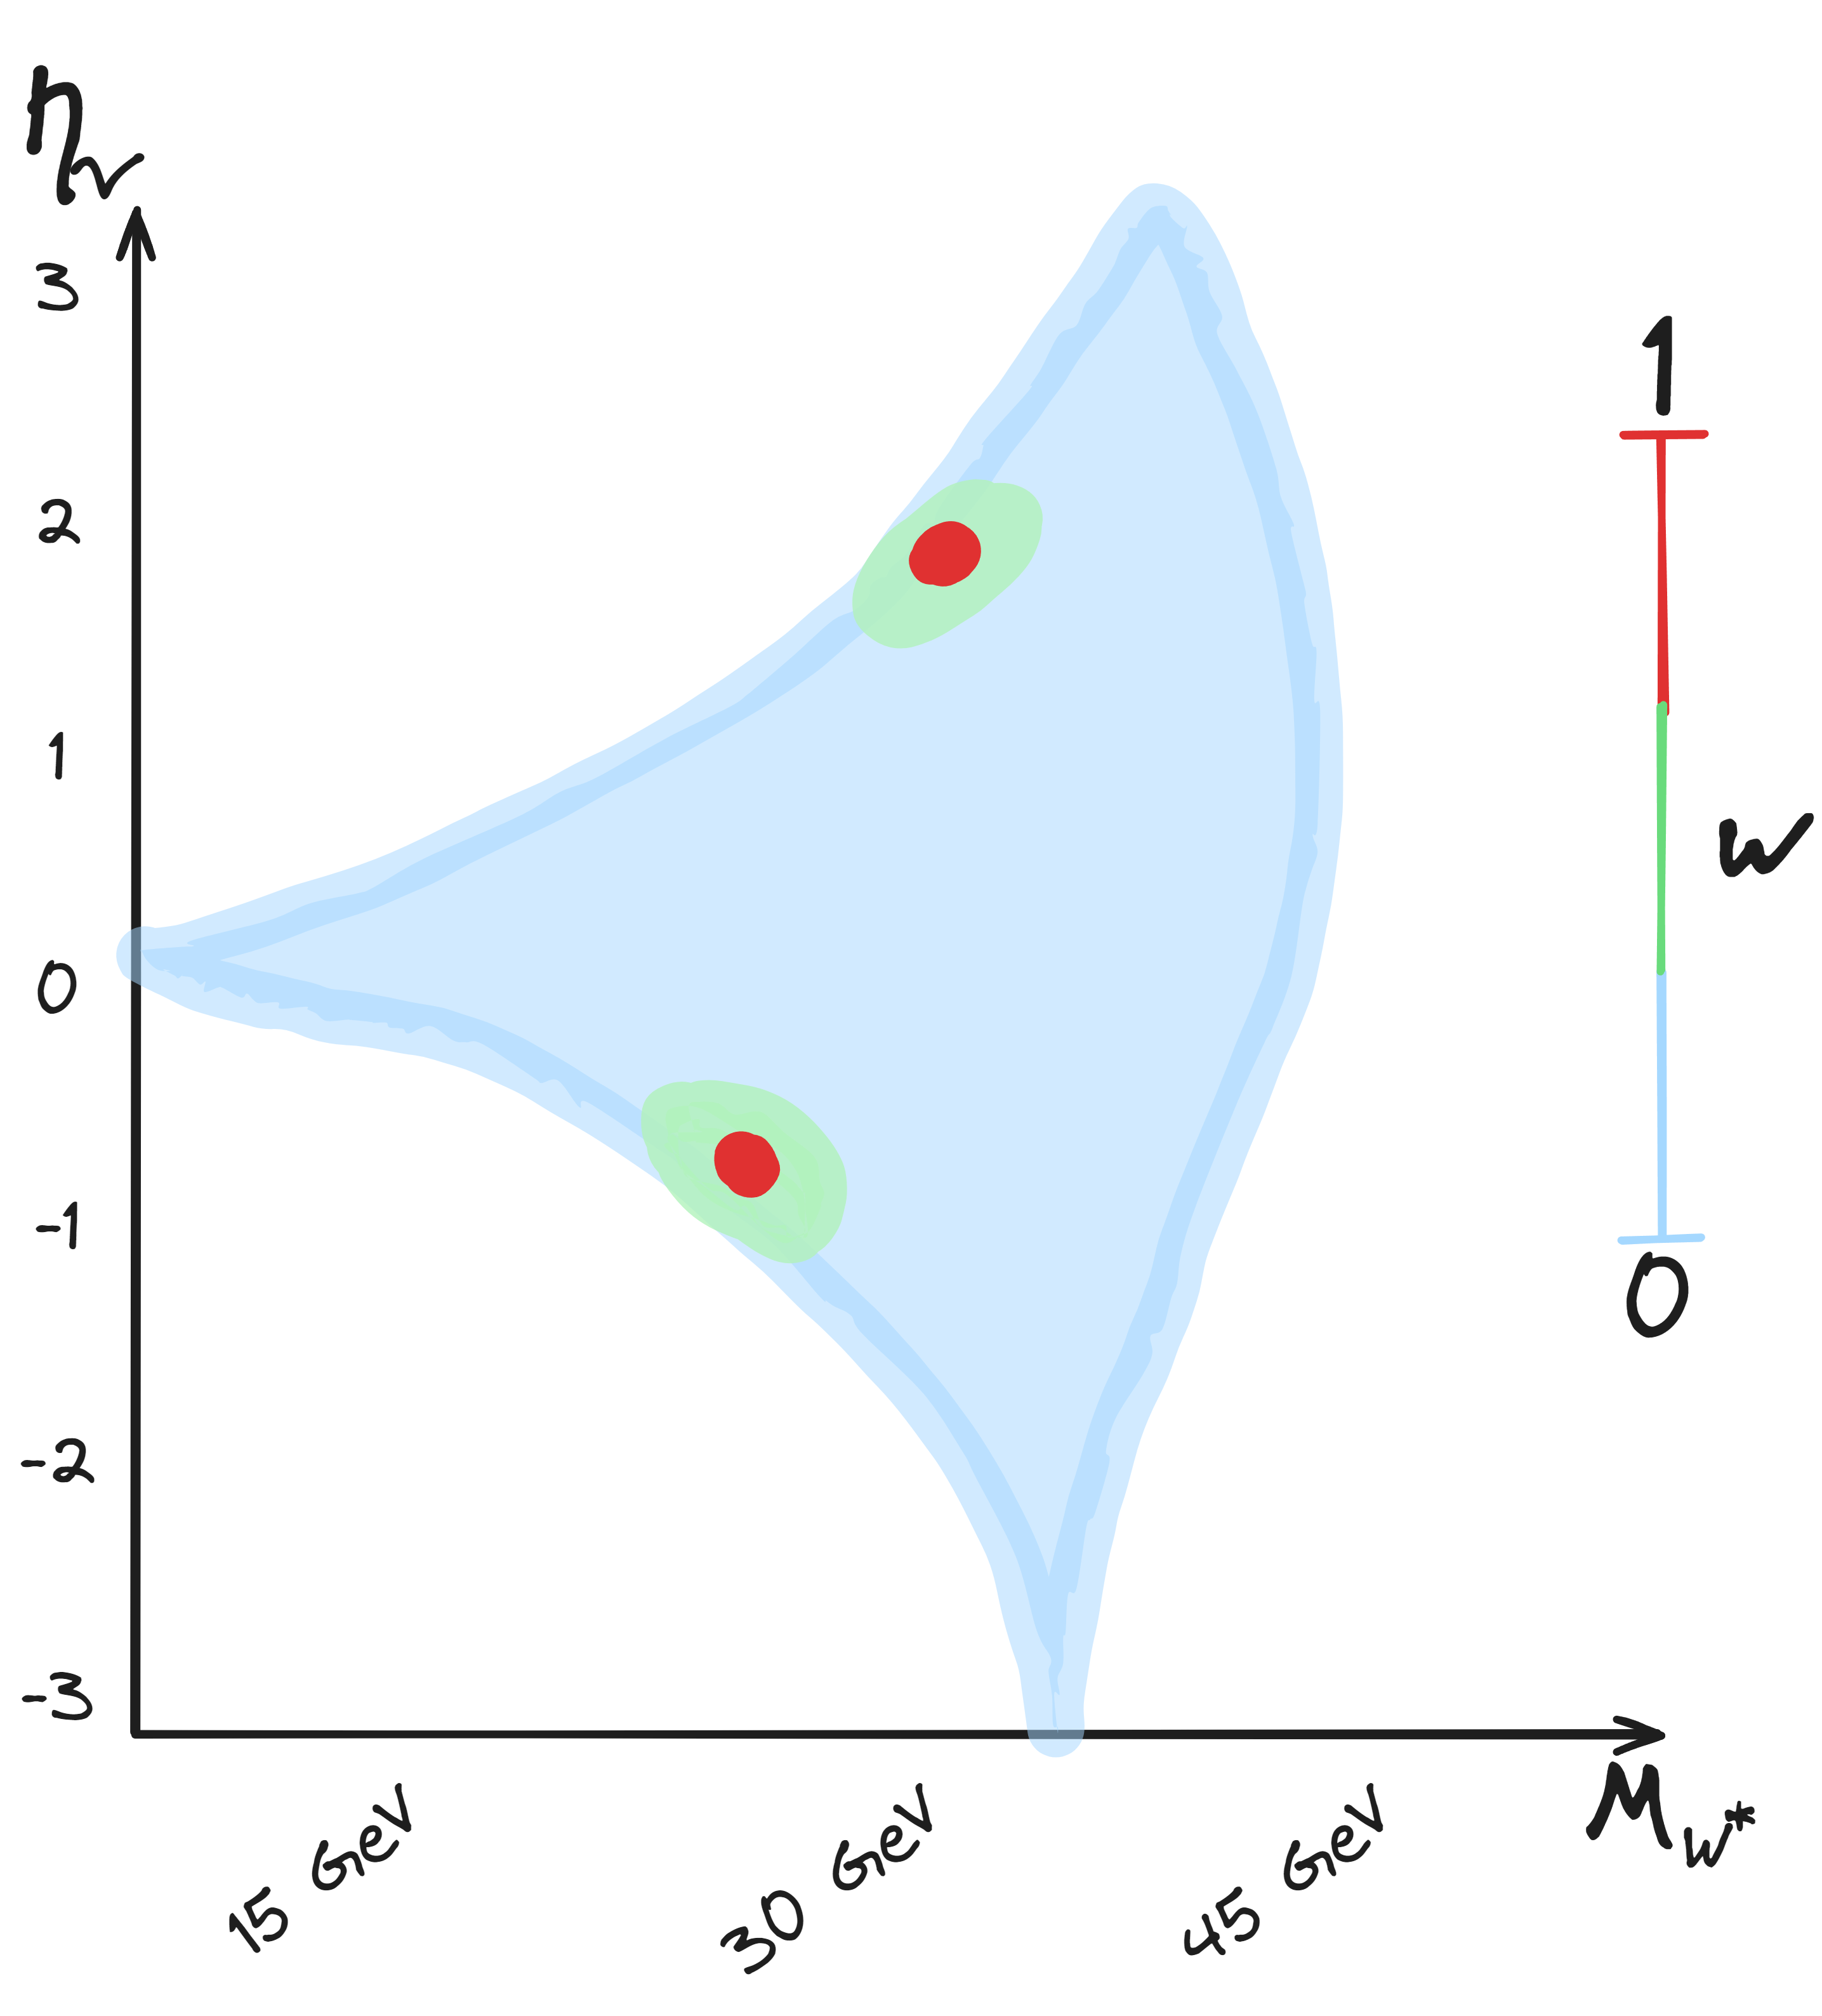
\includegraphics[width=\textwidth]{methods/neutrino_weighting.excalidraw.png}
		\end{figure}
	\end{minipage}
\end{frame}

\begin{frame}{Neutrino Weighting}{Workflow}
	\begin{minipage}{.60\textwidth}
		\begin{itemize}
			\item neutrino weighting yields second prediction
			\begin{itemize}
				\item most likely set of leptonic parameters
			\end{itemize}
			\item full event reconstruction $\Rightarrow$ cross-section measruements
			\begin{itemize}
				\item hadronic prediction by \spanet
				\item leptonic prediction by neutrino weighting
			\end{itemize}
			\item need to implement one step beforehand
			\begin{itemize}
				\item need training samples
			\end{itemize}
		\end{itemize}
	\end{minipage}\hfill
	\begin{minipage}{.2\textwidth}
		\begin{figure}
			\centering
			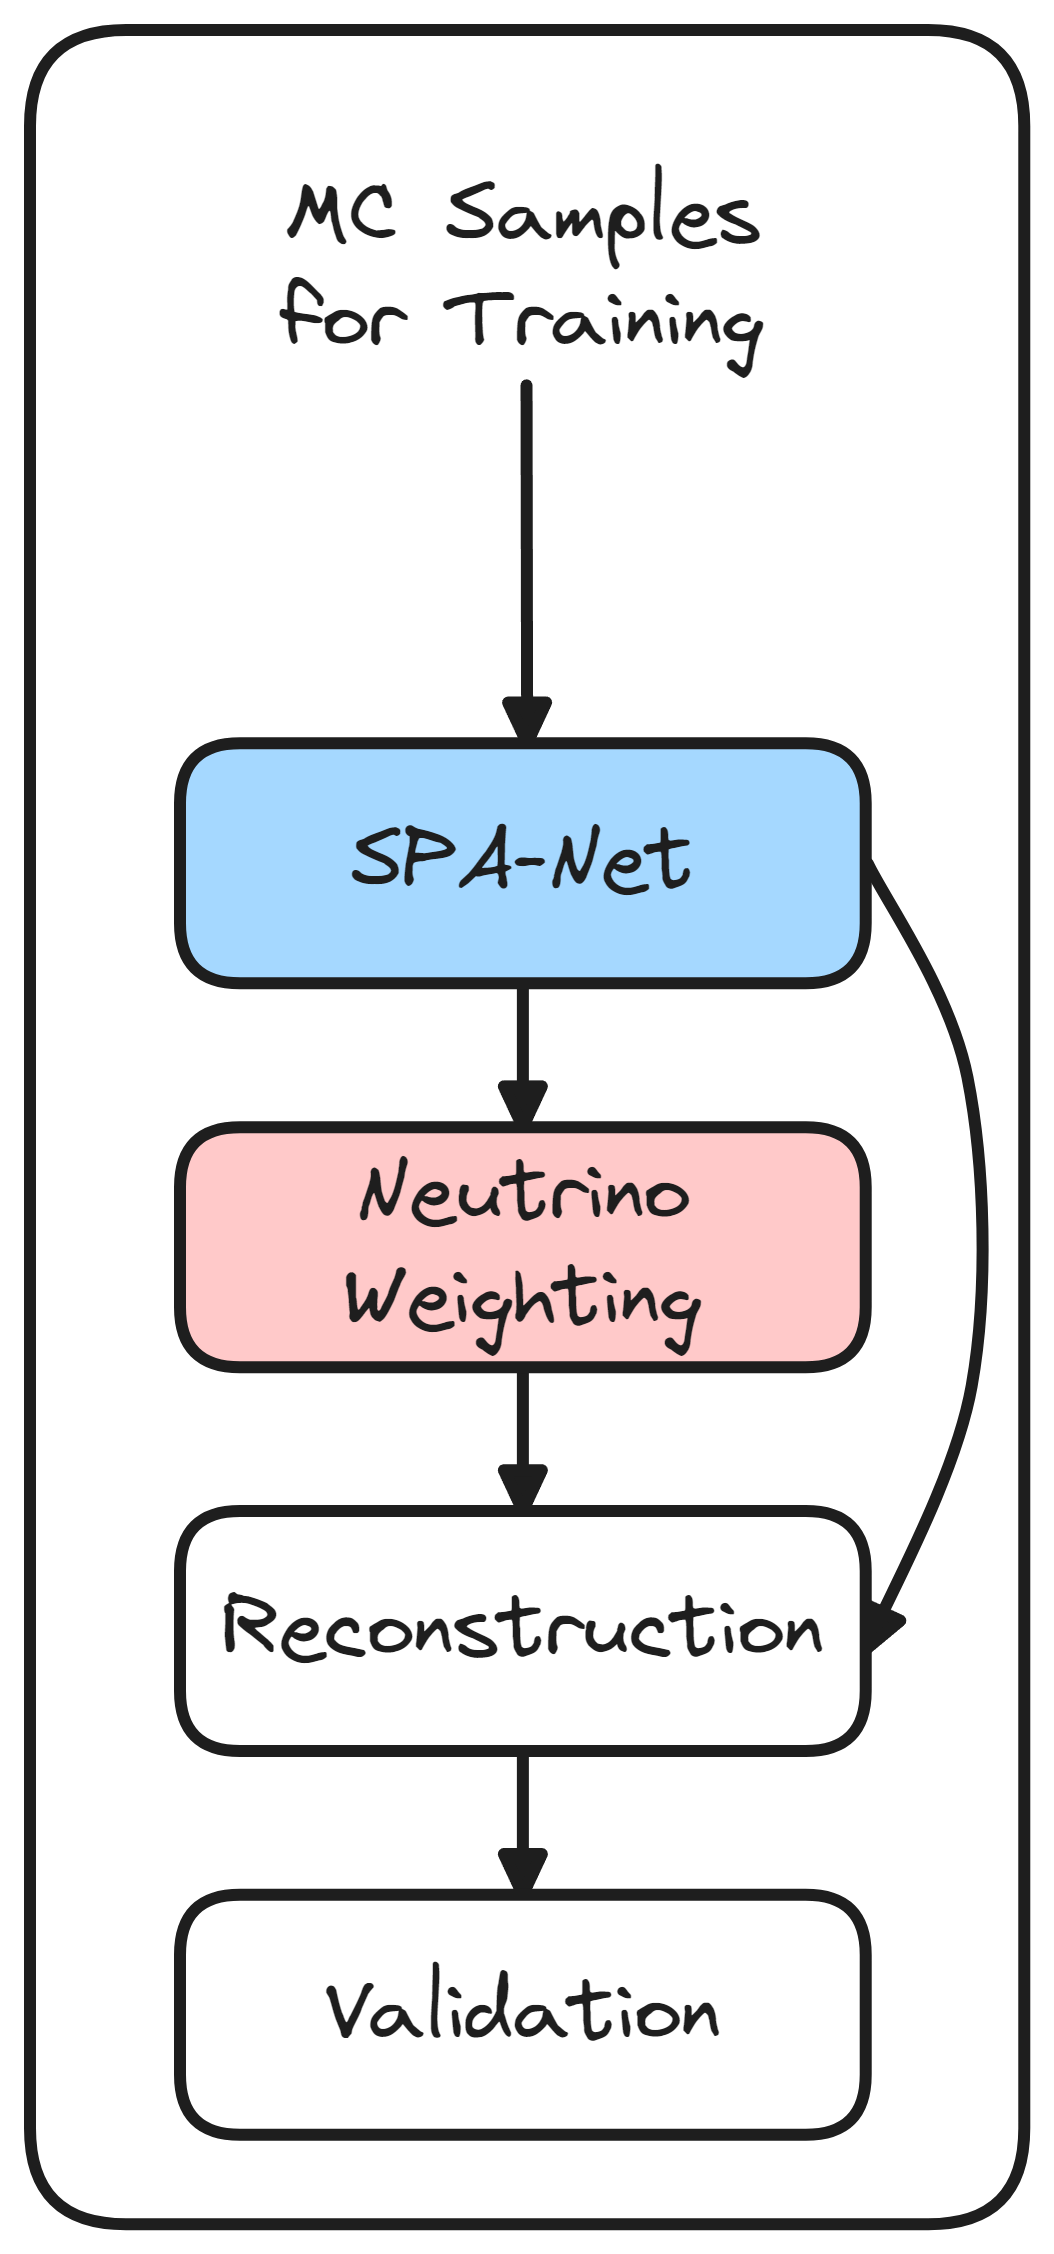
\includegraphics[width=\textwidth]{flowchart/flowchart_f.excalidraw.png}
		\end{figure}
	\end{minipage}
\end{frame}

\begin{frame}{Truth Matching}{Getting Started}
	\begin{minipage}{.75\textwidth}
		\begin{itemize}
			\item truth-matched MC samples unavailable 
			\begin{itemize}
				\item develop custom truth-matching script
			\end{itemize}
			\item currently only \ttbar system is matched 
			\item $W_\text{had}$ not yet matched
			\begin{itemize}
				\item initial plan
				\begin{itemize}
					\item predict \ttbar and \HWW separated
					\item later merge both subsystems
				\end{itemize}
				\item new plan
				\begin{itemize}
					\item also include $W_\text{had}$ from $H$ in \spanet
					\item later merge \spanet with neutrino weighting
				\end{itemize}  
			\end{itemize}
			\item truth matching algorithm can be summarised in 4 steps
		\end{itemize}
	\end{minipage}\hfill
	\begin{minipage}{.2\textwidth}
		\begin{figure}
			\centering
			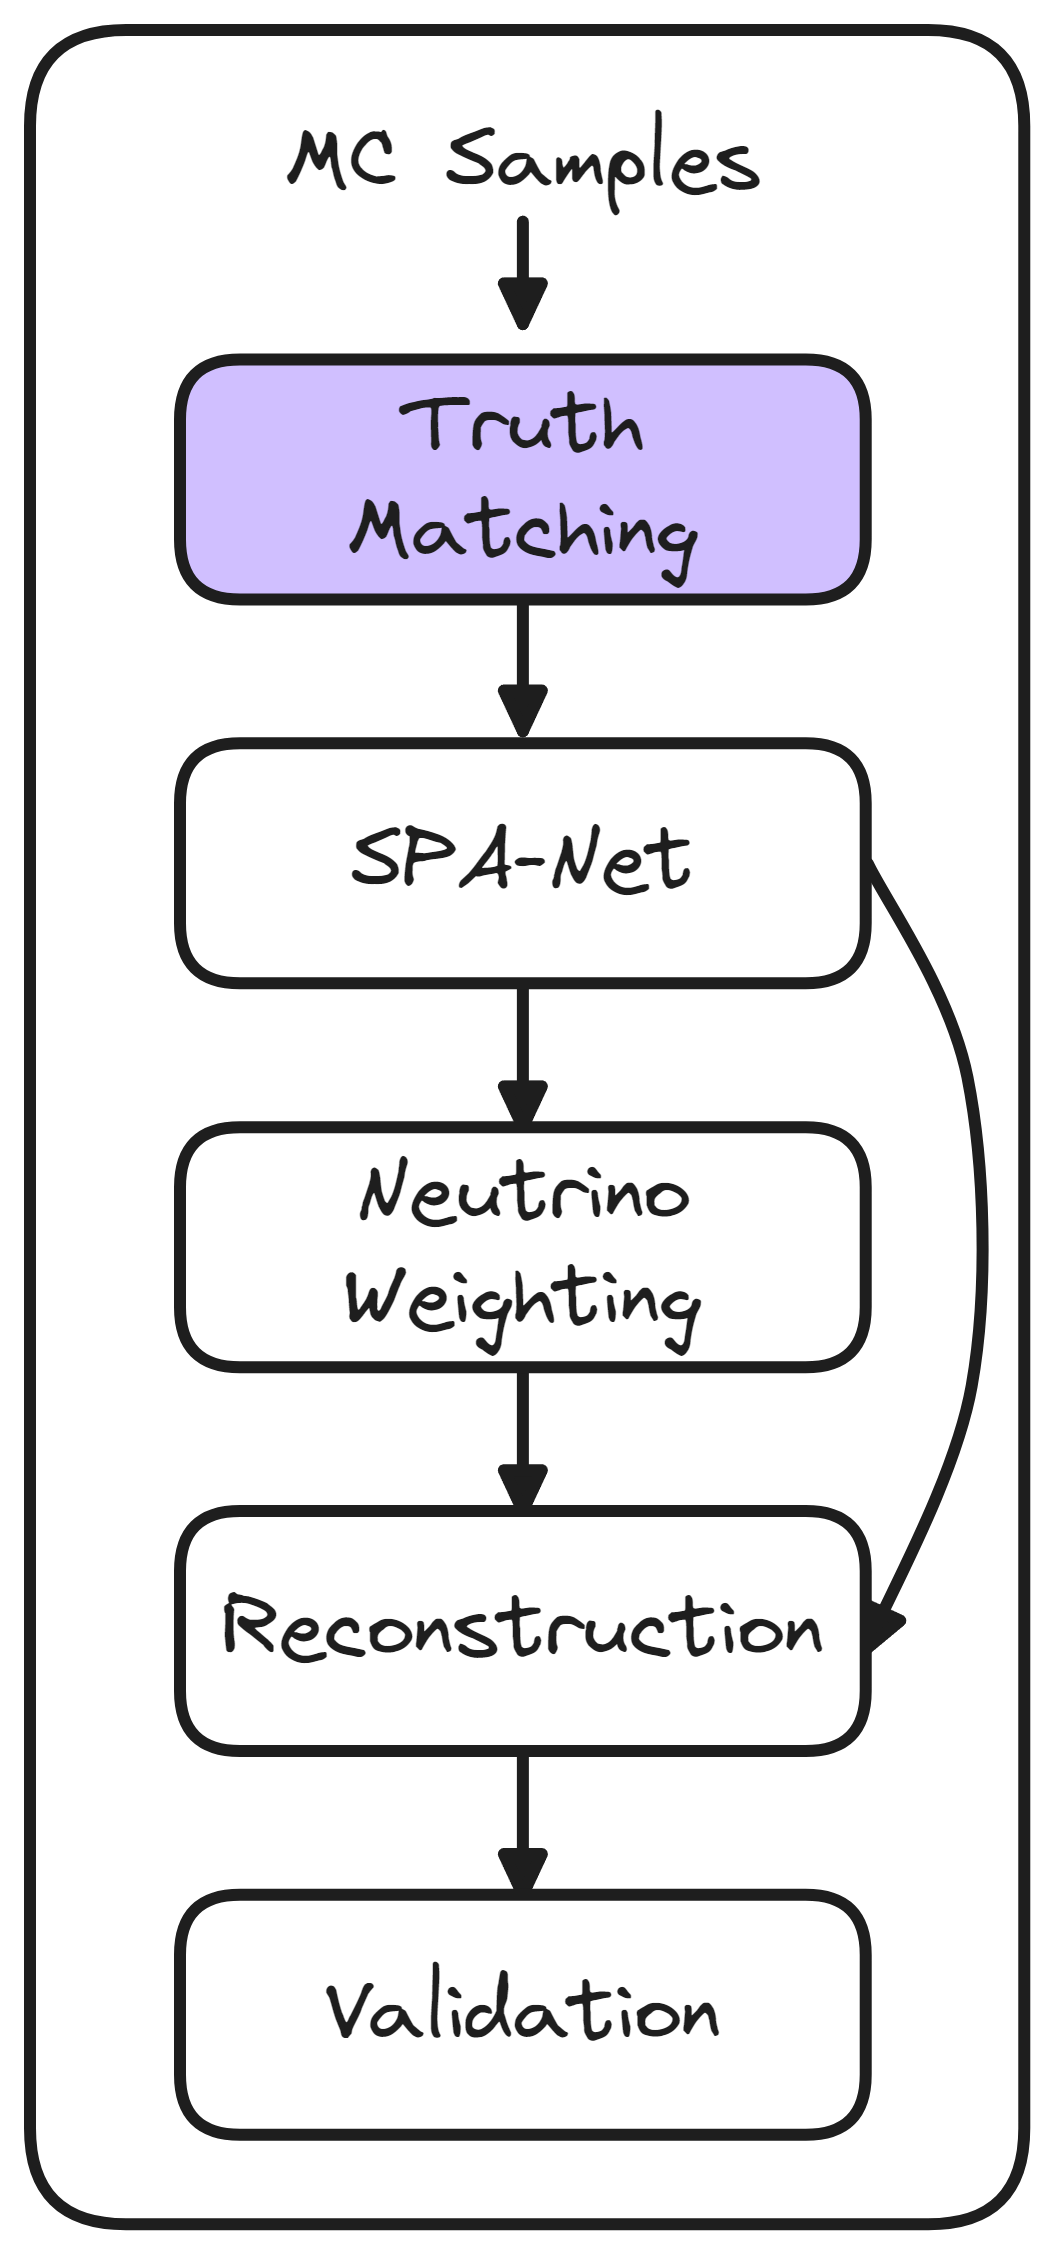
\includegraphics[width=\textwidth]{flowchart/flowchart_b.excalidraw.png}
		\end{figure}
	\end{minipage}
\end{frame}

\begin{frame}{Truth Matching}{The Algorithm in Four Acts}
	\begin{minipage}{.60\textwidth}
		\begin{itemize}
			\item explore $\Delta R$ cone around each truth parton
			\begin{itemize}
				\item search for close \colorbox{red!40}{jets} around each \colorbox{highlighter!40}{truth} parton
				\item 8 partons are expected
				\item limit $\Delta R<0.4$ $\Rightarrow$ overlaps are possible
			\end{itemize}

			\begin{align*}
				\Delta R = \sqrt{\left(\Delta \phi\right)^2 + \left(\Delta \eta\right)^2}
			\end{align*}
		\end{itemize}
	\end{minipage}\hfill
	\begin{minipage}{.38\textwidth}
		\begin{figure}
			\centering
			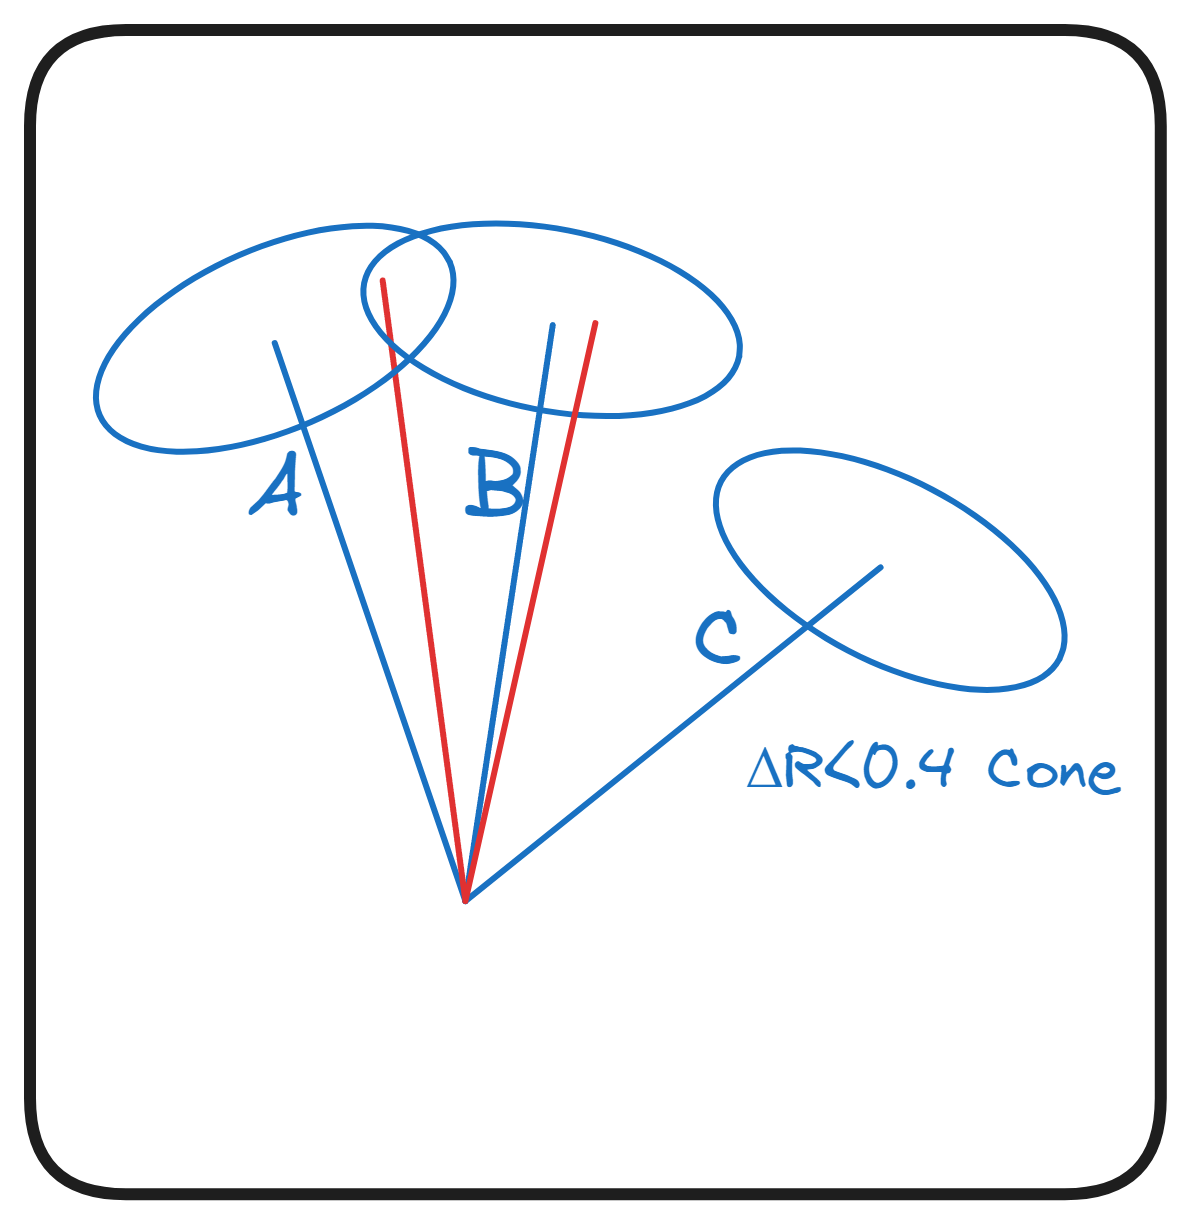
\includegraphics[width=\textwidth]{methods/truth_matching_cones.excalidraw.png}
		\end{figure}
	\end{minipage}
\end{frame}

\addtocounter{framenumber}{-1} 

\begin{frame}{Truth Matching}{The Algorithm in Four Acts}
	\begin{minipage}{.60\textwidth}
		\begin{itemize}
			\item explore $\Delta R$ cone around each truth parton 
			\item identify valid jet matches within cone
			\begin{itemize}
				\item all jets within each cone are valid
				\item save potential matches for each parton
			\end{itemize}
		\end{itemize}
	\end{minipage}\hfill
	\begin{minipage}{.38\textwidth}
		\begin{figure}
			\centering
			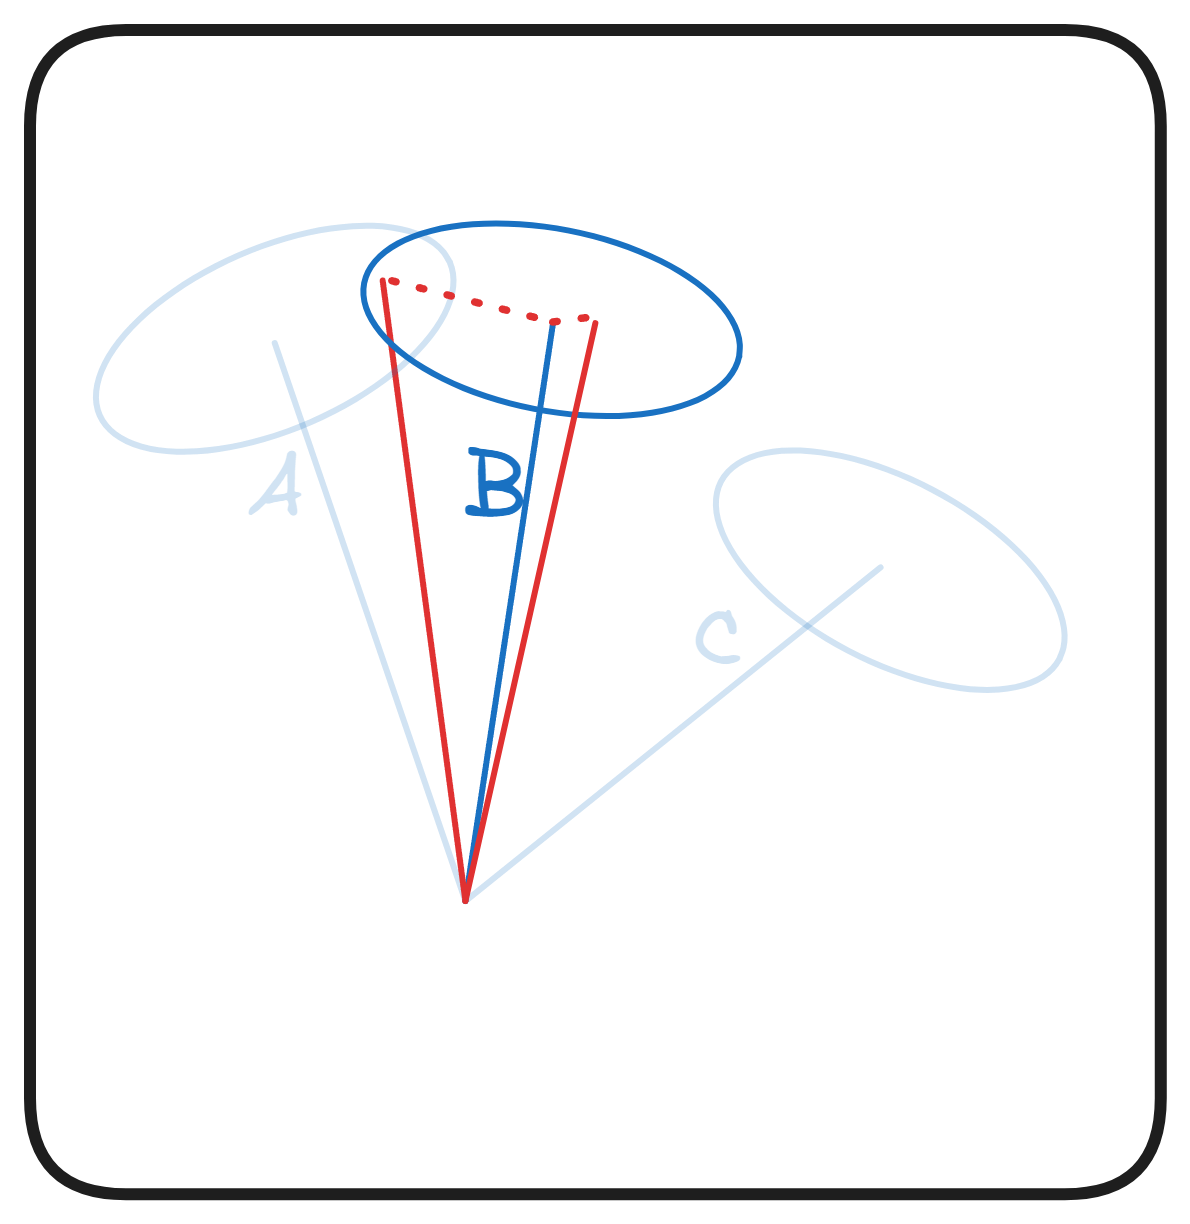
\includegraphics[width=\textwidth]{methods/truth_matching_potential.excalidraw.png}
		\end{figure}
	\end{minipage}
\end{frame}

\addtocounter{framenumber}{-1} 

\begin{frame}{Truth Matching}{The Algorithm in Four Acts}
	\begin{minipage}{.60\textwidth}
		\begin{itemize}
			\item explore $\Delta R$ cone around each truth parton 
			\item identify valid jet matches within cone
			\item decide a final match for each truth parton 
			\begin{itemize}
				\item multiple potential matches possible
				\item different schemes were tested
			\end{itemize}
		\end{itemize}
	\end{minipage}\hfill
	\begin{minipage}{.38\textwidth}
		\begin{figure}
			\centering
			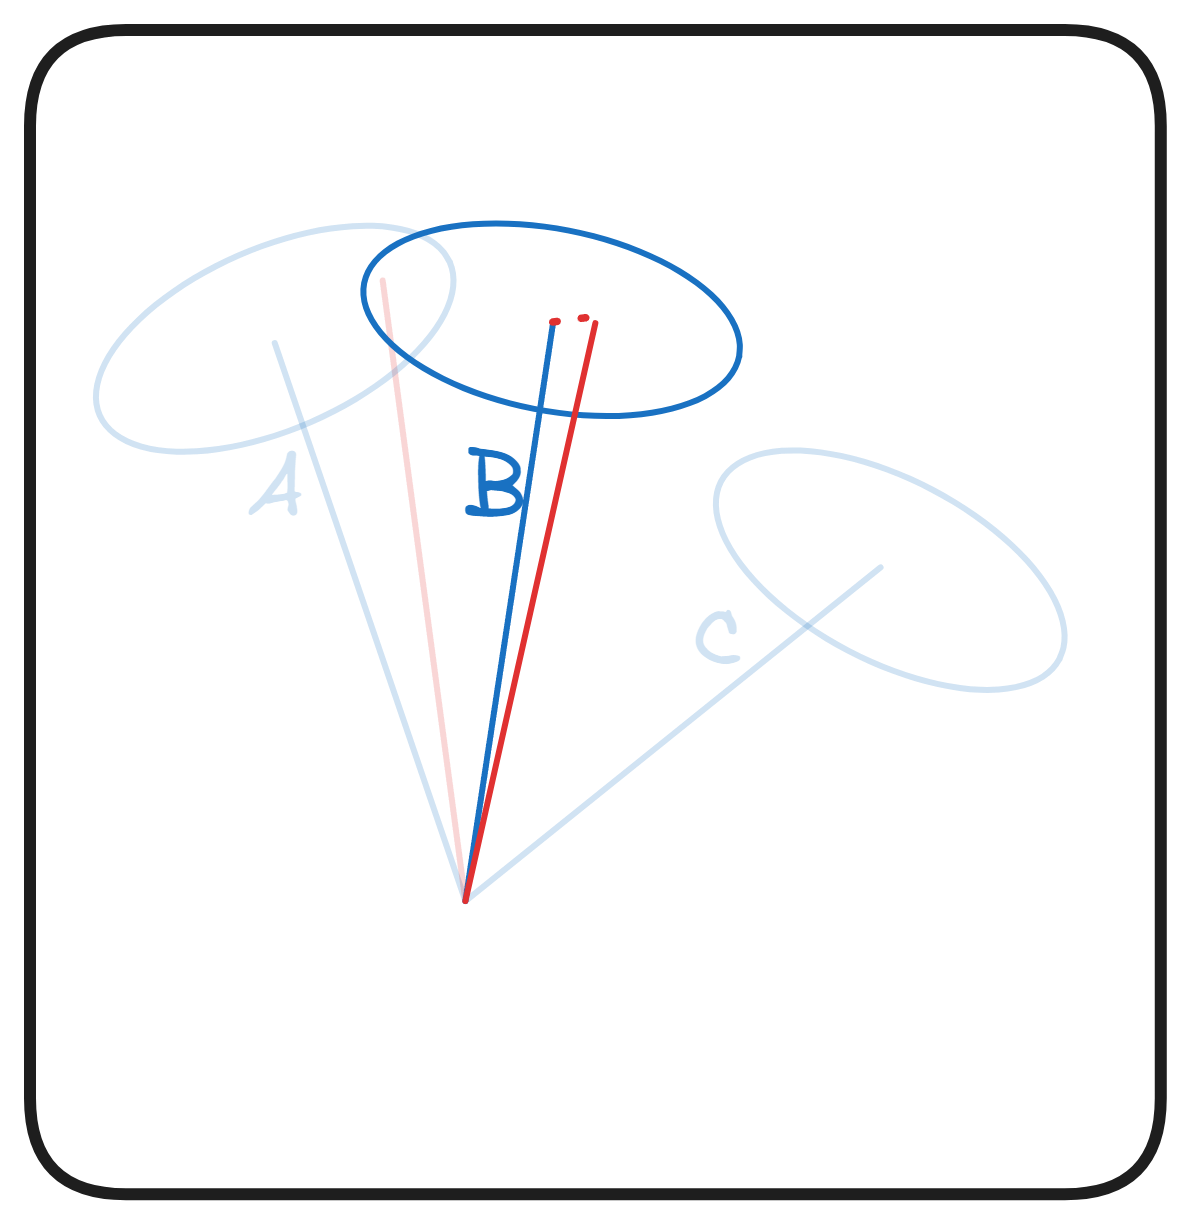
\includegraphics[width=\textwidth]{methods/truth_matching_final1.excalidraw.png}
		\end{figure}
	\end{minipage}
\end{frame}

\addtocounter{framenumber}{-1} 

\begin{frame}{Truth Matching}{The Algorithm in Four Acts}
	\begin{minipage}{.60\textwidth}
		\begin{itemize}
			\item explore $\Delta R$ cone around each truth parton 
			\item identify valid jet matches within cone
			\item decide a final match for each truth parton 
			\item repeat the process
			\begin{itemize}
				\item matched jets are unavailable for others
				\item try to find match for each truth parton
				\item partial reconstruction possible $\Rightarrow$ still use in \spanet
			\end{itemize}
		\end{itemize}
	\end{minipage}\hfill
	\begin{minipage}{.38\textwidth}
		\begin{figure}
			\centering
			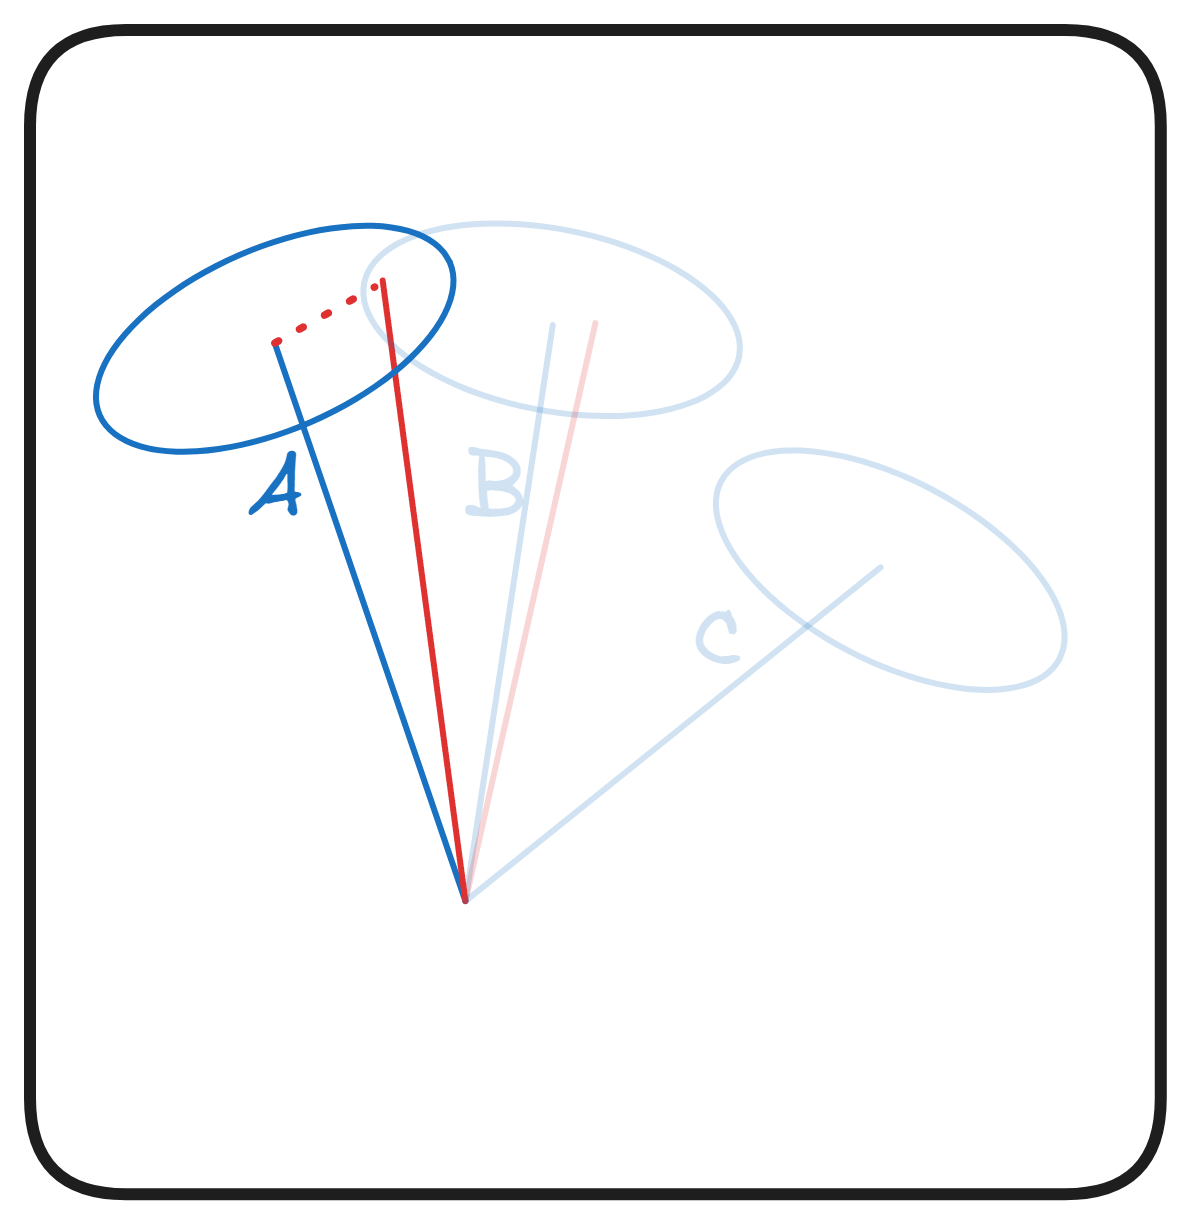
\includegraphics[width=\textwidth]{methods/truth_matching_final2.excalidraw.png}
		\end{figure}
	\end{minipage}
\end{frame}


% \begin{frame}{Results}{How Many Jets are Matched}
% 	\begin{minipage}{.43\textwidth}
% 		\begin{itemize}
% 			\item overview: matched jets multiplicities (using 1M events)
% 			\begin{itemize}
% 				\item most events can match only 
% 				\item note that \spanet training can utilise partial events 
% 				\item limit at 6 for \ttbar (8  hadronic $W$)
% 			\end{itemize}
% 		\end{itemize}
% 	\end{minipage}\hfill
% 	\begin{minipage}{.45\textwidth}
% 		\begin{figure}
% 			\centering
% 			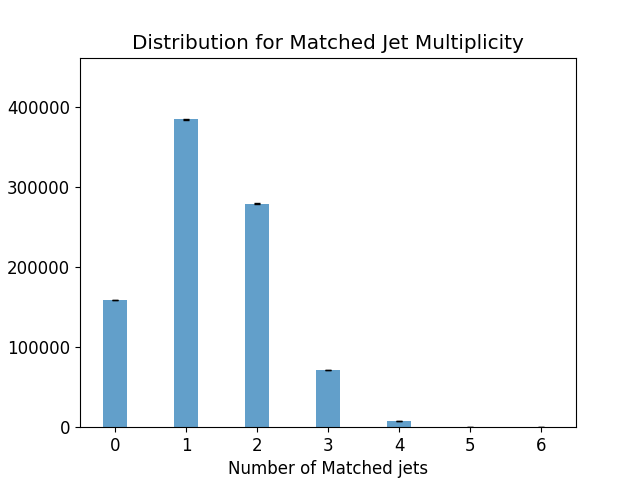
\includegraphics[width=\textwidth]{results/matched_jets.png}
% 		\end{figure}
% 	\end{minipage}
% \end{frame}

\begin{frame}{Results}{Match Full \ttbar System}
	\begin{itemize}
		\item investigate complete \ttbar matches
		\begin{itemize}
			\item 8 jets needed for \ttbar and hadronic $W_\text{hadronic}$
			\item high jet multiplicity $\Rightarrow$ increased success but lower statistics (due to NLO)
	  	\end{itemize}
	\end{itemize}
	\begin{figure}
		\centering
		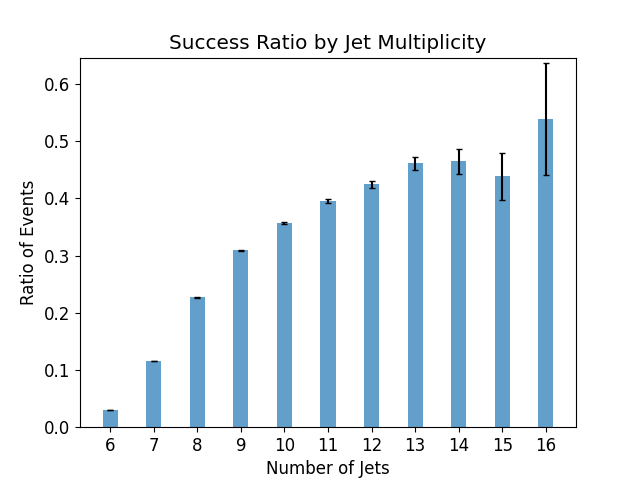
\includegraphics[width=.4\textwidth]{results/success_ratio.png}\hspace{.02\textwidth}
		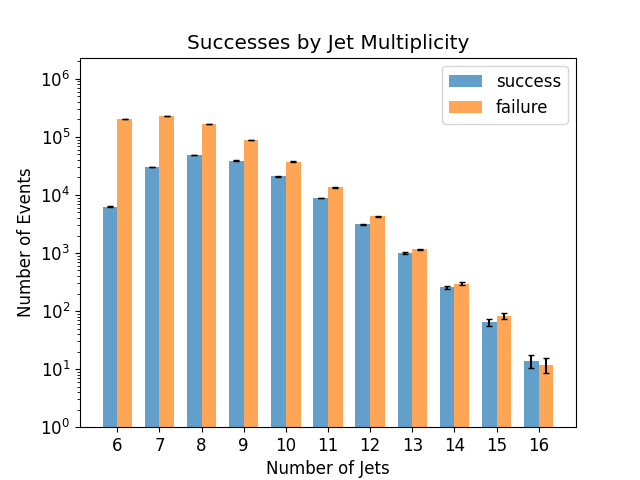
\includegraphics[width=.4\textwidth]{results/success_by_jets.png}
	\end{figure}
\end{frame}

\begin{frame}{Results}{The Final Selection Scheme}
	\begin{itemize}
    	\item testing $\Delta R$ and $\Delta p_T$ information %($W$ parity violation $\Rightarrow$ $p_T$ beneficial?)  %violation => not same pt in quarks )
    	\begin{itemize}
			\item single: $\Delta R$ (or $\Delta p_T$) only
			\begin{itemize}
		  		\item look for the closest jet in $\eta$-$\phi$ (or $p_T$) to parton
			\end{itemize}
			\item hybrid: $\Delta R$ + $\Delta p_T$
			\begin{itemize}
				\item scale $\Delta R$ and $\Delta p_T$ to same range
			\end{itemize}
		\end{itemize}
    	\item no improvement over $\Delta R$ only
    	\begin{itemize}
      		\item $\sim$20\% events with 2+ potential matches $\Rightarrow$ most events are unaffected
			\item $\Delta R$ only performs best and will be used (no further investigation)
    	\end{itemize}
	\end{itemize}

	\begin{table}
		\centering
		\begin{tabular}{l|c|c|c|c|c|}
			&\multicolumn{5}{c|}{successful matching in \%}\\
			& $t\bar{t}$ & $t$ & $\bar{t}$ & $W_t$ & $\bar{W_t}$\\
			\hline
			\rowcolor{highlighter!40}
			$\Delta R$ only & 17.6 & 43.9 & 44.1 & 53.4 & 53.6\\
			$\Delta R$ + $\Delta p_T$ & 17.5 & 43.7 & 43.9 & 53.1 & 53.2\\
			$\Delta p_T$ only & 17.4 & 43.6 & 43.9 & 53.0 & 53.2\\
		\end{tabular}
	\end{table}
\end{frame}

\begin{frame}{Results}{Inspecting Different Regions}
	\begin{itemize}
		\item regions by jet multiplicity + $H$ decay mode
		\begin{itemize}
			\item yields relative to full sample 
			\item semileptonic \HWW of special interest
		\end{itemize}
		\item truth record pdgID bug prevents selecting 90\% events $\Rightarrow$ low statistics for \HWW
		\item fully hadronic \HWW excluded due to single-lepton triggers and broken truth record
	\end{itemize}

	\begin{table}
		\centering
		\begin{tabular}{l|r|c|c|c|c|c|}
			&&\multicolumn{5}{c|}{successful matches in \%}\\
			& rel. yield & $t\bar{t}$ & $t$ & $\bar{t}$ & $W_t$ & $\bar{W_t}$\\
			\hline
			$(\text{all})^{\text{5+ jets}}$  & 100.0\% & 15.8 & 41.0 & 41.2 & 50.5 & 50.7\\
			$(\text{all})^{\text{6+ jets}}$  & 90.1\% & 17.6 & 43.9 & 44.1 & 53.4 & 53.6\\
			$(\text{all})^{\text{8+ jets}}$  & 5.2\% & 30.1 & 56.3 & 56.5 & 62.9 & 63.1\\
			\hline
			$(H\rightarrow bb)^{\text{8+ jets}}$ & 27.4\% & 27.3 & 53.9 & 54.0 & 63.4 & 63.4\\
			$(\HWW)^{\text{8+ jets}}$ & 0.52\% & 31.2 & 56.9 & 57.4 & 63.6 & 63.8\\
			\hline
			$(\HWW)_{\text{fully leptonic}}^{\text{8+ jets}}$ & 0.41\% & 31.6 & 57.3 & 57.8 & 64.0 & 64.2\\
			\rowcolor{highlighter!40}
			$(\HWW)_{\text{semileptonic}}^{\text{8+ jets}}$ & 0.11\% & 29.6 & 55.4 & 55.8 & 62.2 & 62.3\\
			$(\HWW)_{\text{fully hadronic}}^{\text{8+ jets}}$ & 0.00\% & - & - & - & - & -\\
		\end{tabular}
	\end{table}
\end{frame}

\begin{frame}{Conclusion}{Summary}
	\begin{minipage}{.75\textwidth}
		\begin{itemize}
			\item current status   
			\begin{itemize}
				\item using MC input
				\item truth-matching for training samples
				\item training/fine-tuning \spanet for hadronic predictions
			\end{itemize}
			\item next steps
			\begin{itemize}
				\item implement neutrino weighting for leptonic predictions
				\item full event reconstruction
				\item validate reconstruction
			\end{itemize}
		\end{itemize}
	\end{minipage}\hfill
	\begin{minipage}{.2\textwidth}
		\begin{figure}
			\centering
			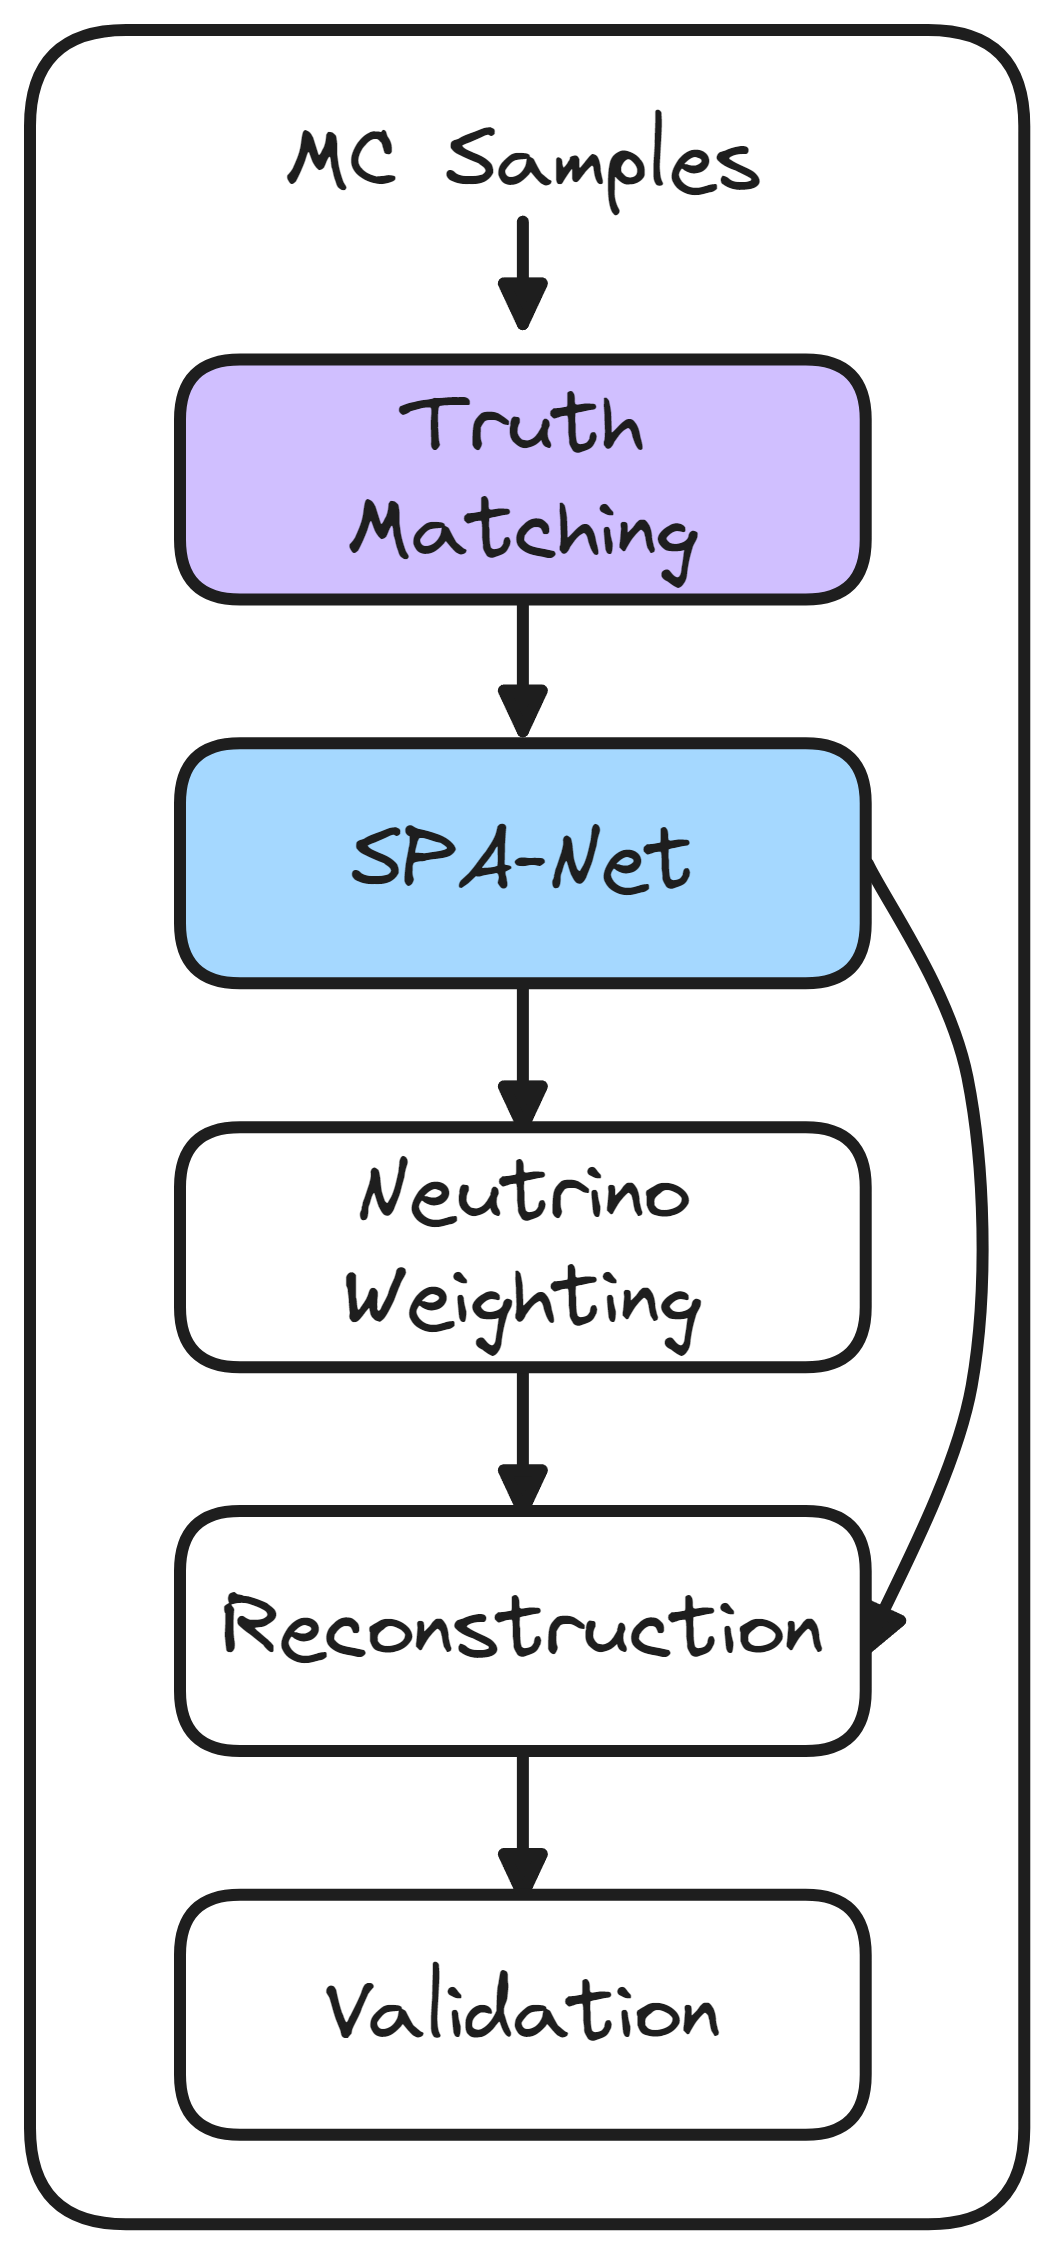
\includegraphics[width=\textwidth]{flowchart/flowchart_h.excalidraw.png}
		\end{figure}
	\end{minipage}
\end{frame}

\addtocounter{framenumber}{-1} 

\begin{frame}{Conclusion}{Summary}
	\begin{minipage}{.75\textwidth}
		\begin{itemize}
			\item switch to real data
			\begin{itemize}
				\item predictions by \spanet + neutrino weighting
				\item background suppression using neutrino weighting 
				\item cross-section (and other) measurements
			\end{itemize}
		\end{itemize}
	\end{minipage}\hfill
	\begin{minipage}{.2\textwidth}
		\begin{figure}
			\centering
			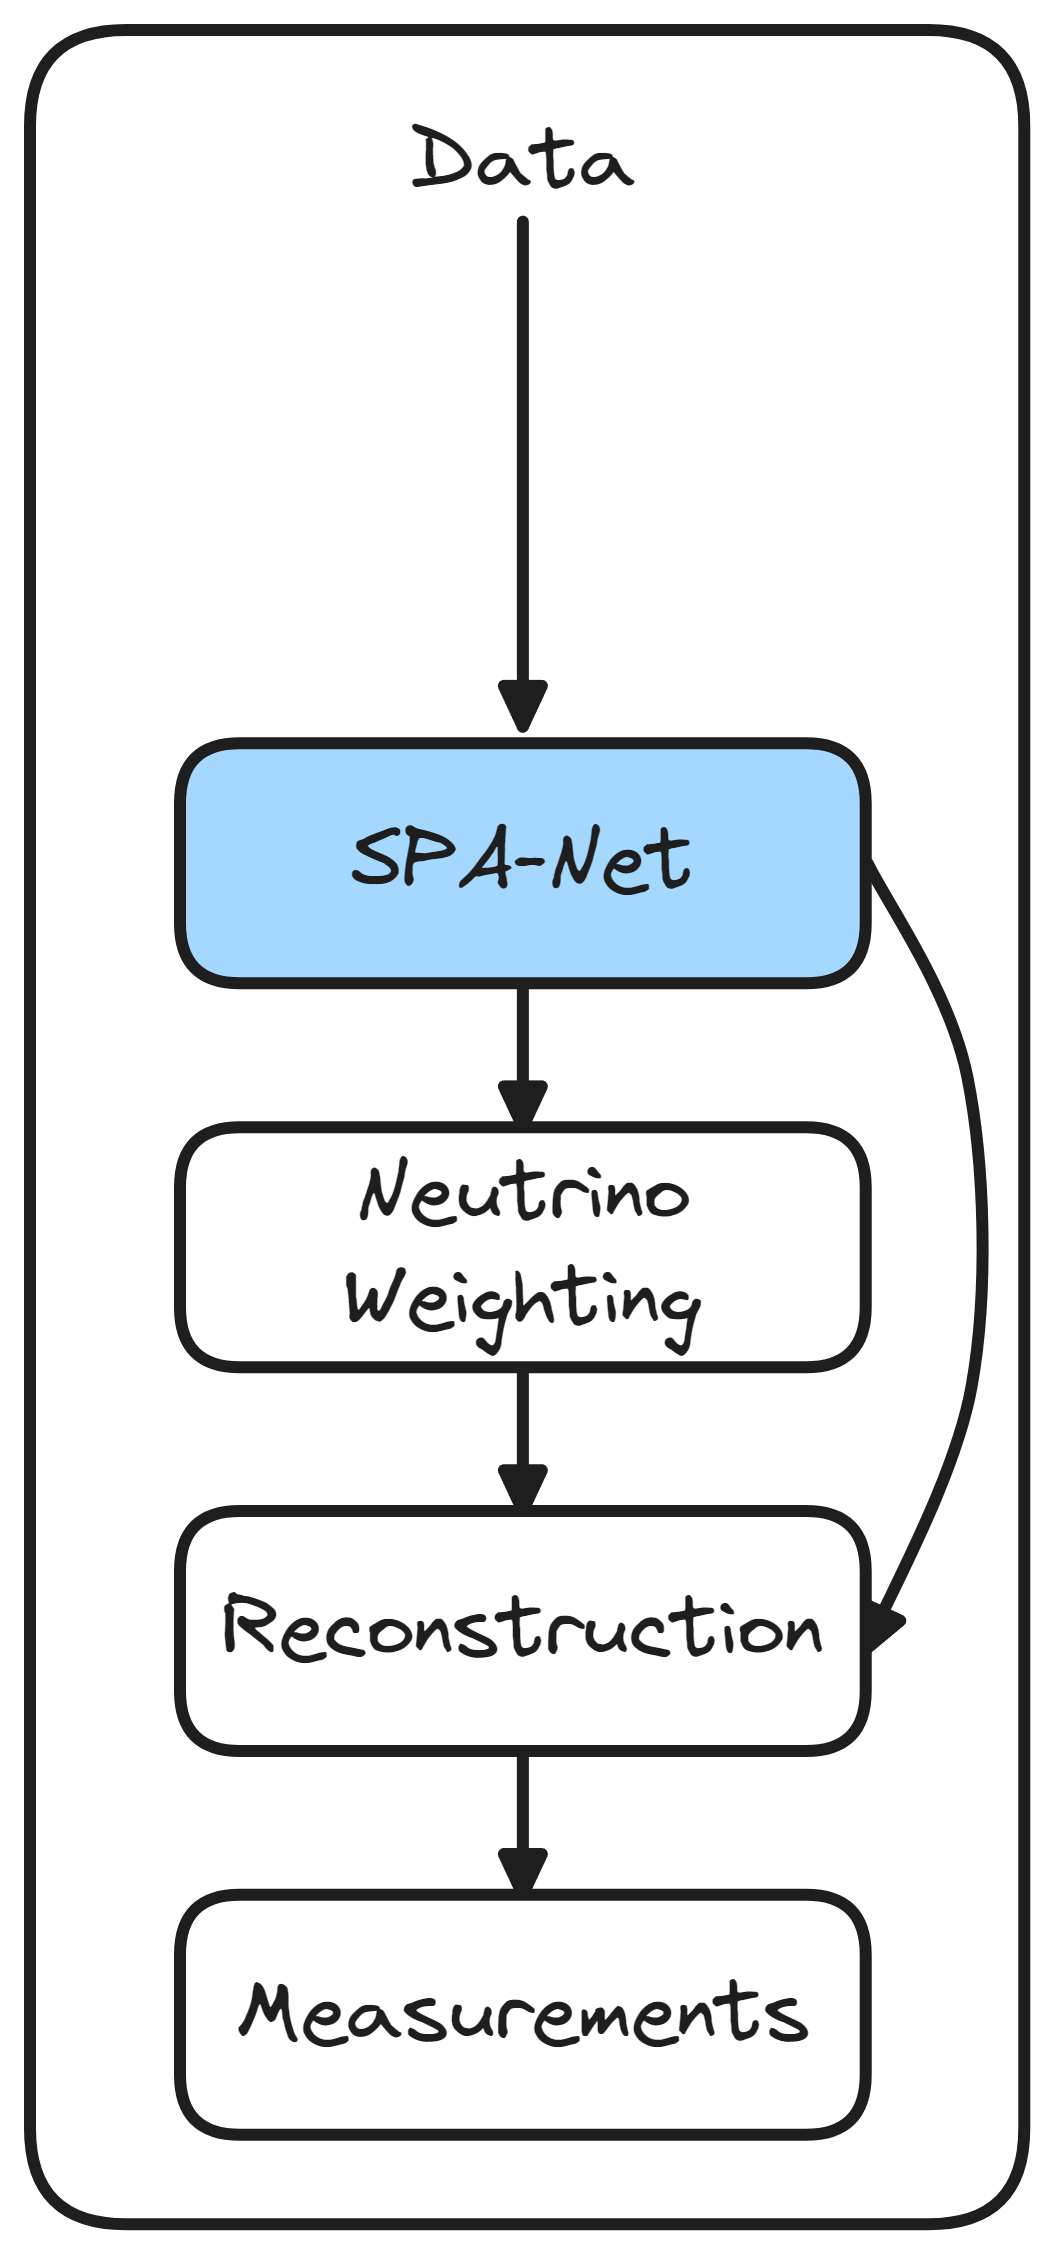
\includegraphics[width=\textwidth]{flowchart/flowchart_g.excalidraw.png}
		\end{figure}
	\end{minipage}
\end{frame}

\begin{frame}{Conclusion}{Roadmap}
	\begin{itemize}
		\item currently in the 5th month (project start: 3rd November)
		\begin{itemize}
			\item[\ding{51}] develop, validate and refine truth matching
			\item[\ding{51}] setup training environment on NAF (\desy)
			\item[\ding{51}] successfully run first \spanet training jobs
			\item[!] finishing the half-time report
			\item[!] rework truth matching (add hadronic $W$ from $H$) $\Rightarrow$ new training samples 
			\item[!] fine-tune \spanet
			\item[o] implement neutrino weighting
			\item[o] merge for full event reconstruction
			\item[o] test background suppression
			\item[o] switch to real data
			\item[o] cross-section measurements + expand analysis
			% \item SM investigations ($tH$ coupling, $H$ decay ratio,...)
			% \item compare $\chi^2$ vs \spanet (performance, precision, resources)
		\end{itemize}
	\end{itemize}

	\vspace{10mm}

	\begin{center}
    	\color{highlighter}\textbf{\LARGE Thanks for your attention!}
  	\end{center}
\end{frame}


% =======================================================
% =======  BACKUP  ======================================
% =======================================================
\appendix

\begin{frame}{Background}{Feynman diagrams}
	\begin{itemize}
		\item feynman diagrams for $t\bar{t}Z$ and $t\bar{t}W$ background signatures
	\end{itemize}

	\begin{figure}
		\centering
		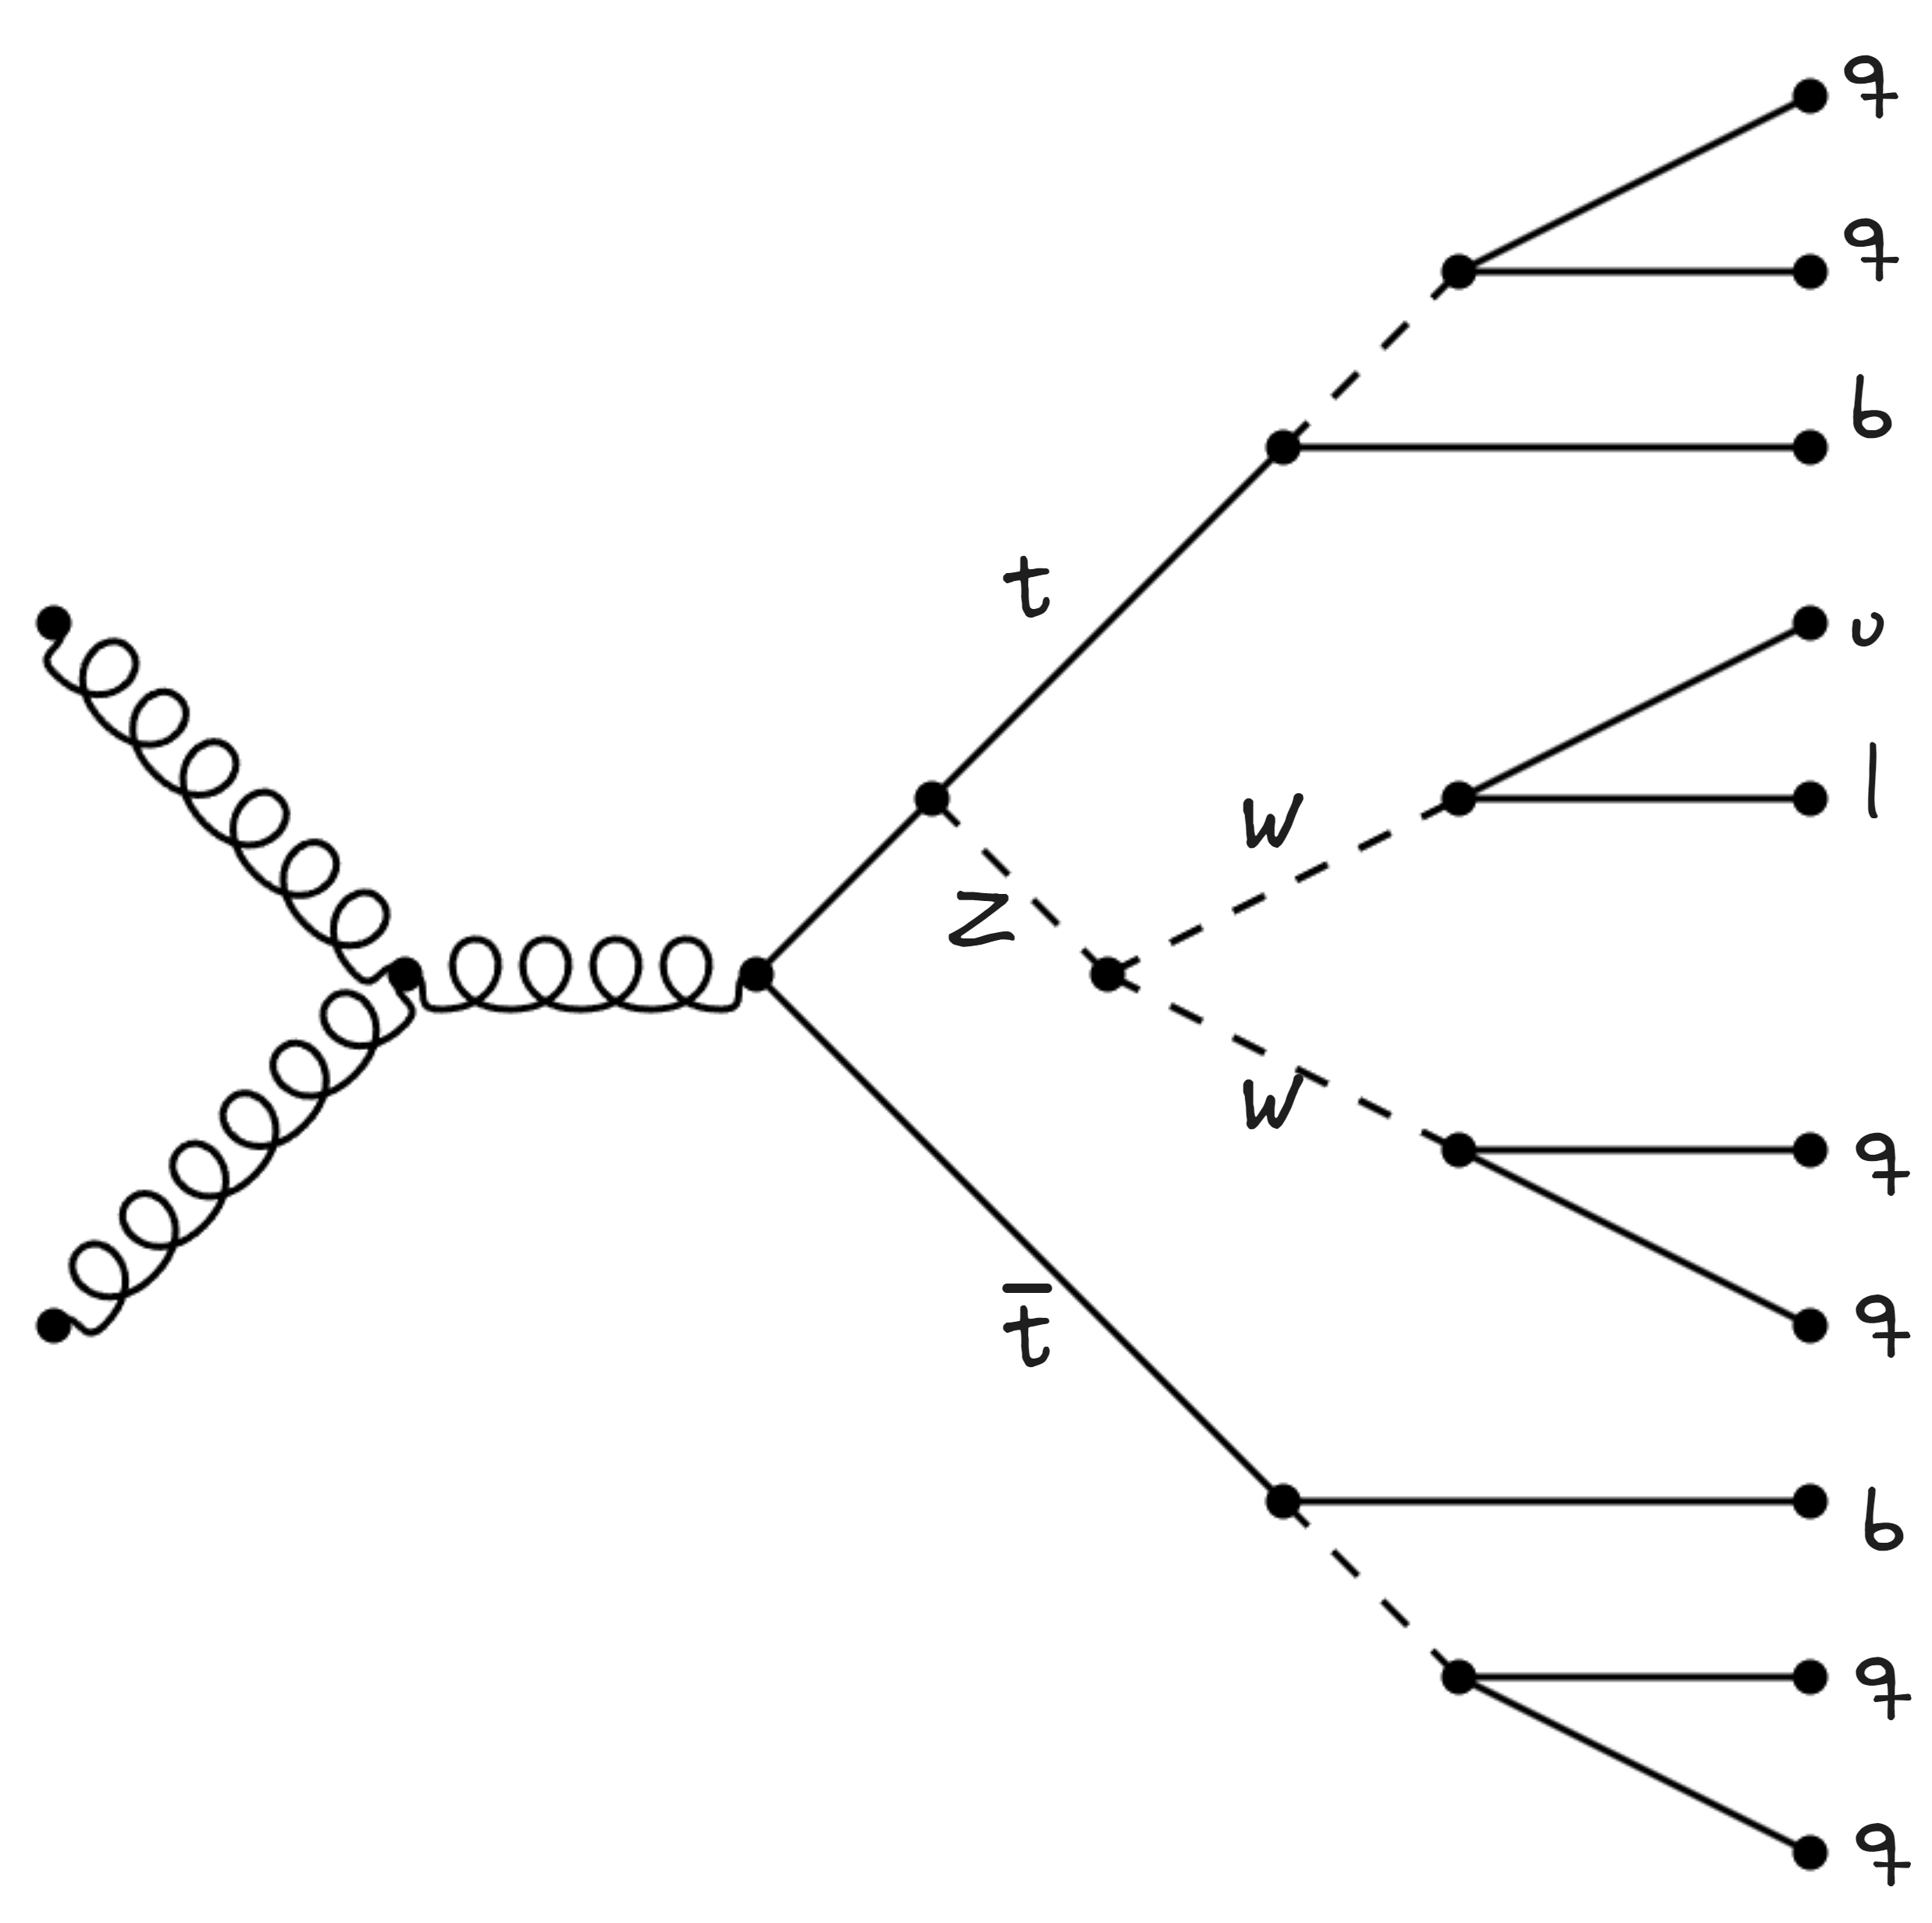
\includegraphics[width=.35\textwidth]{feynman_diagrams/background_ttzww.excalidraw.png}\hspace{10mm}
		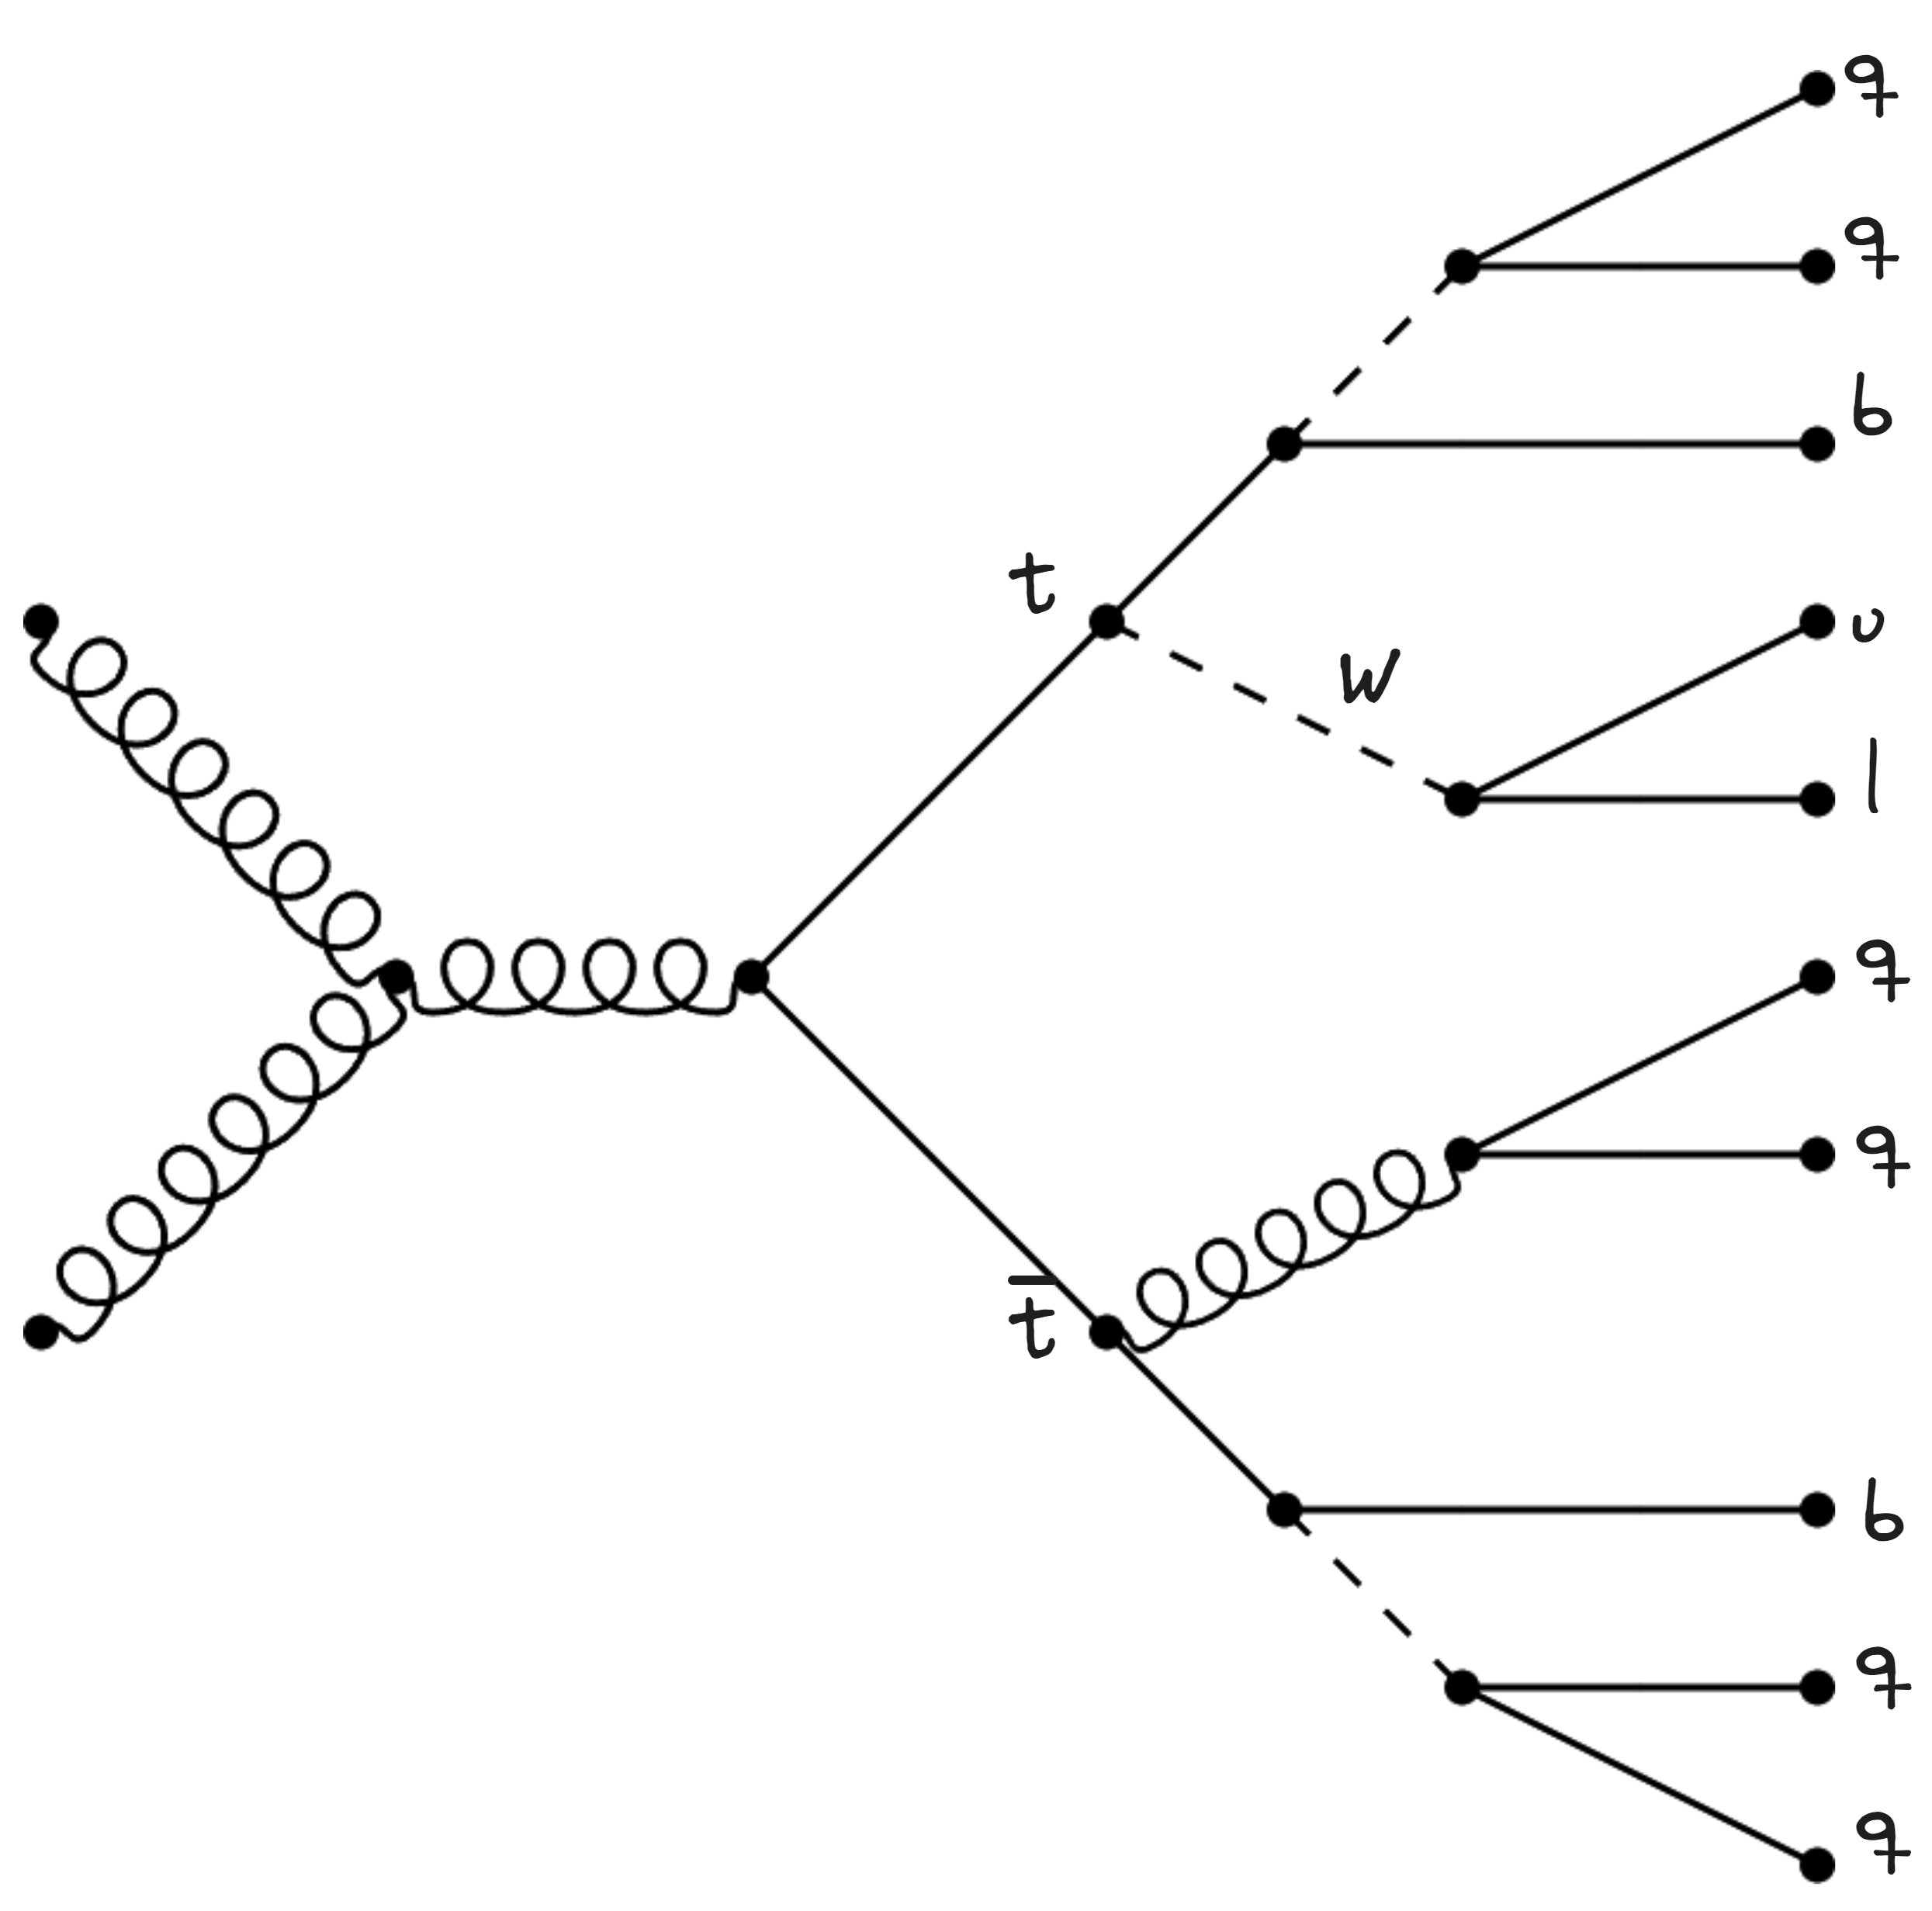
\includegraphics[width=.35\textwidth]{feynman_diagrams/background_ttwg.excalidraw.png}
	\end{figure}
\end{frame}

\begin{frame}{Truth Matching}{Technical Details}
	\begin{minipage}{.69\textwidth}
		\begin{itemize}
			\item low resources $\Rightarrow$ can run locally
			\begin{itemize}
				\item save matches efficiently as integers 
				\item utilise fast bit shifting operations
			\end{itemize}
			\item local runtime (1M events) 
			\begin{itemize}
				\item $\sim$30\,s matching
				\item $\sim$2.4\,h conversion
			\end{itemize}
			\item bottleneck is .root $\rightarrow$ .hd5 conversion
			\begin{itemize}
				\item fixing array size + generating a mask
				\item only needed once per training sample
			\end{itemize}
		\end{itemize}
	\end{minipage}\hfill
	\begin{minipage}{.3\textwidth}
		\begin{figure}
			\centering
			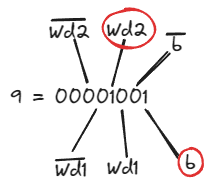
\includegraphics[width=\textwidth]{methods/truth_matching_binary.png}
		\end{figure}
	\end{minipage}
\end{frame}

\begin{frame}{SPA-Net}{The Algorithm}
    \begin{itemize}
		\item divide assignment problem into sub-problems
		\begin{itemize}
			\item solve each resonance particle individually
			\item utilise 'Symmetric Tensor Attention'
			\begin{itemize}
				\item input: encoded jets
				\item apply some complicated tensor transformer (enforcing no self-combinations)
				\item output: tensor $\mathcal{P}$ $\Rightarrow$ probabilities for each valid combination
				\item preserves jet symmetries + allows partial event reconstructions
			\end{itemize}
 		\end{itemize}
		\item combine sub-problems
		\begin{itemize}
			\item acquire final jet-parton assignment
			\item utilise 'Combined Symmetric Loss'
			\begin{itemize}
				\item input: probability tensors $\mathcal{P}_i$ + true $\delta_i$ distributions
				\item calculate cross entropy for each sub-problem
				\item output: final assignment with minimal loss (for all equivalent labels)  
				\item preserves particle symmetries
			\end{itemize}
		\end{itemize}
	\end{itemize}
\end{frame}

\begin{frame}{SPA-Net}{Jet symmetries}
	\begin{itemize}
		\item $k$ partons for each resonance particle $p$
		\item jet symmetries implemented as permutation group $G=\{\forall\sigma\in G | \mathcal{P}^{j_1...j_k} = \mathcal{P}^{j_{\sigma(1)}...j_{\sigma(k)}}\}$
		\item $\mathcal{X}$: transformer-encoded jets
		\item $\Theta$: trained parameter tensor of output layer
		\item $\mathcal{S}$: $G$-symmetric tensor constructed from $\Theta$
		\item $\mathcal{O}$: extended $\mathcal{S}$ representing $k$ similarities in input sequence
		\item $\mathcal{P}$: normalised output tensor $\mathcal{O}$ $\Leftrightarrow$ $\sum\mathcal{P}_p=1$
	\end{itemize}

	\begin{align*}
		\mathcal{S}^{i_1...i_k} &= \sum_{\sigma\in G_p} \Theta^{i_{\sigma(1)}...i_{\sigma(k)}}\\
		\mathcal{O}^{j_1...j_k} &= \prod_{a=1}^{k} \mathcal{X}_{i_a}^{j_a} \cdot \mathcal{S}^{i_1...i_k}\\
		\mathcal{P}^{j_1...j_k} &= \frac{\exp\left(\mathcal{O}^{j_1...j_k}\right)}{\sum_{j_1...j_k}\exp\left(\mathcal{O}^{j_1...j_k}\right)}
	\end{align*}
\end{frame}

\end{document}
